\section{実験結果}
\subsection{粘度計測}
鋼球落下実験を行う試験溶液として,1wt.\%PAA溶液の製作を行った.この製作した溶液の粘度特性を確認し,先行研究\cite{ref:9}\cite{ref:10}における粘度特性と比較した.この比較を行うことで先行研究との粘度特性の違いを確認した.なお,この粘度計測を実施するためには,溶質が溶媒に十分に均一に溶解することならびに,混合時に混入した気泡がおおむね消失することが必要であるため,溶液製作1週間後に行った.それぞれの試料に対し,円錐回転子の回転数を変化させ,各5回計測を行いその平均を求めた.

水道水の粘度計測を行った結果をFig.\ref{fig:water-vis}に示す.なお,縦軸は粘度,横軸はせん断速度を表す.2.2においても示したが,コーンロータの回転速度を変化させることにより,せん断速度を変化させた.その結果,粘度は約1.1[Pa$\times$ s]でほぼ一定となっていた.これは,水がニュートン流体であり,粘度を比例係数とした速度勾配とせん断応力の比例関係となっているためであると考えられる.

水道水の場合と同様にPAA溶液の粘度計測を行った結果をFig.\ref{fig:PAA-vis}に示す.なお,縦軸は粘度の対数,横軸はせん断速度の対数を表す.また,Iwamuro {\it et al.}\cite{ref:9}やShiratori {\it et al.}\cite{ref:10}の文献値も共に示した.ここで,粘度$\mu$はせん断速度$\dot{\gamma}$に対して,粘度定数 k[Pa$\times$ $\text{s}^n$],指数$n$を用い Power-law modelに従うものとすると,
\begin{eqnarray}
    \label{eq:power-low}
    \mu=k\times\dot{\gamma}^{n-1}
\end{eqnarray}
といった式で与えられる\cite{ref:1}.式\ref{eq:power-low}を用いて近似線計算を行った結果,$k$=7.39[Pa$\times \text{s}^n]$,$n=0.23$であった.Iwamuro {\it et al.}\cite{ref:9}では,$k$=9.4[Pa$\times \text{s}^n]$,$n=0.23$と示されている.また,Shiratori {\it et al.}\cite{ref:10}を同様に解析すると,$k$=4.7[Pa$\times \text{s}^n$],$n=0.18$となっていた.今回作製したPAA溶液の粘度特性はIwamuro {\it et al.}とShiratori {\it et al.}の間に位置しており,適切に作製されたと判断できる.

\begin{figure}[ht]
    \centering
    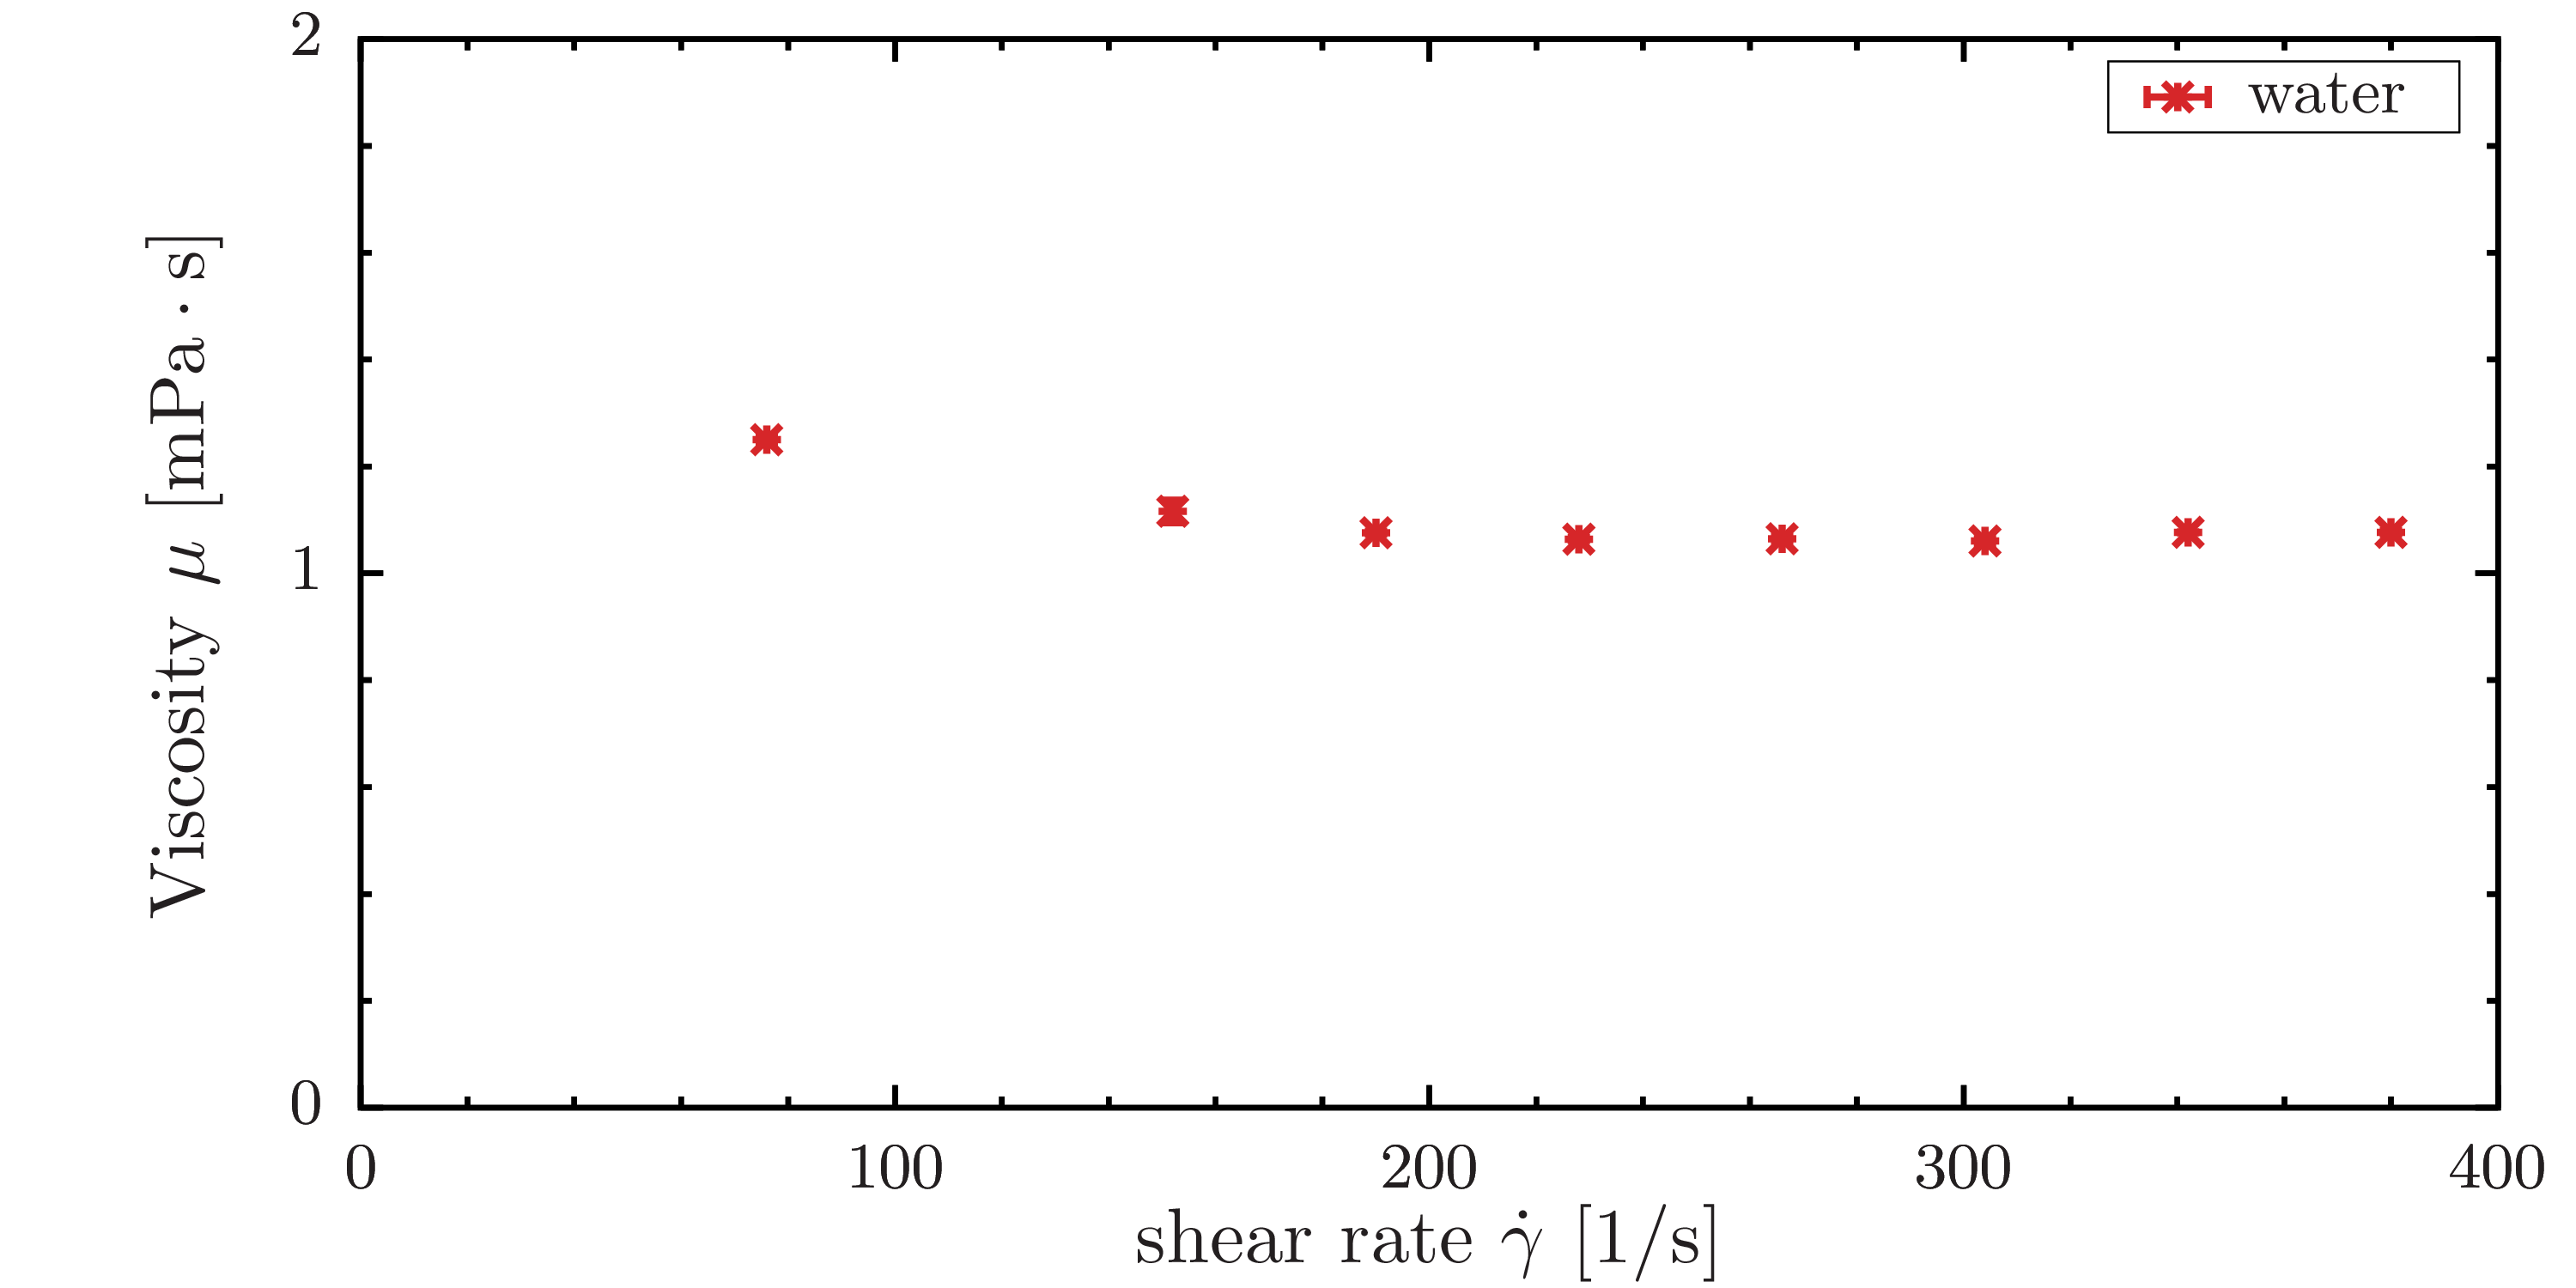
\includegraphics[width=12cm,clip]{4-Results/water.png}
    \caption{Meansured viscosity versus shear rate for tap water.}
    \label{fig:water-vis}
\end{figure}

\begin{figure}[ht]
    \centering
    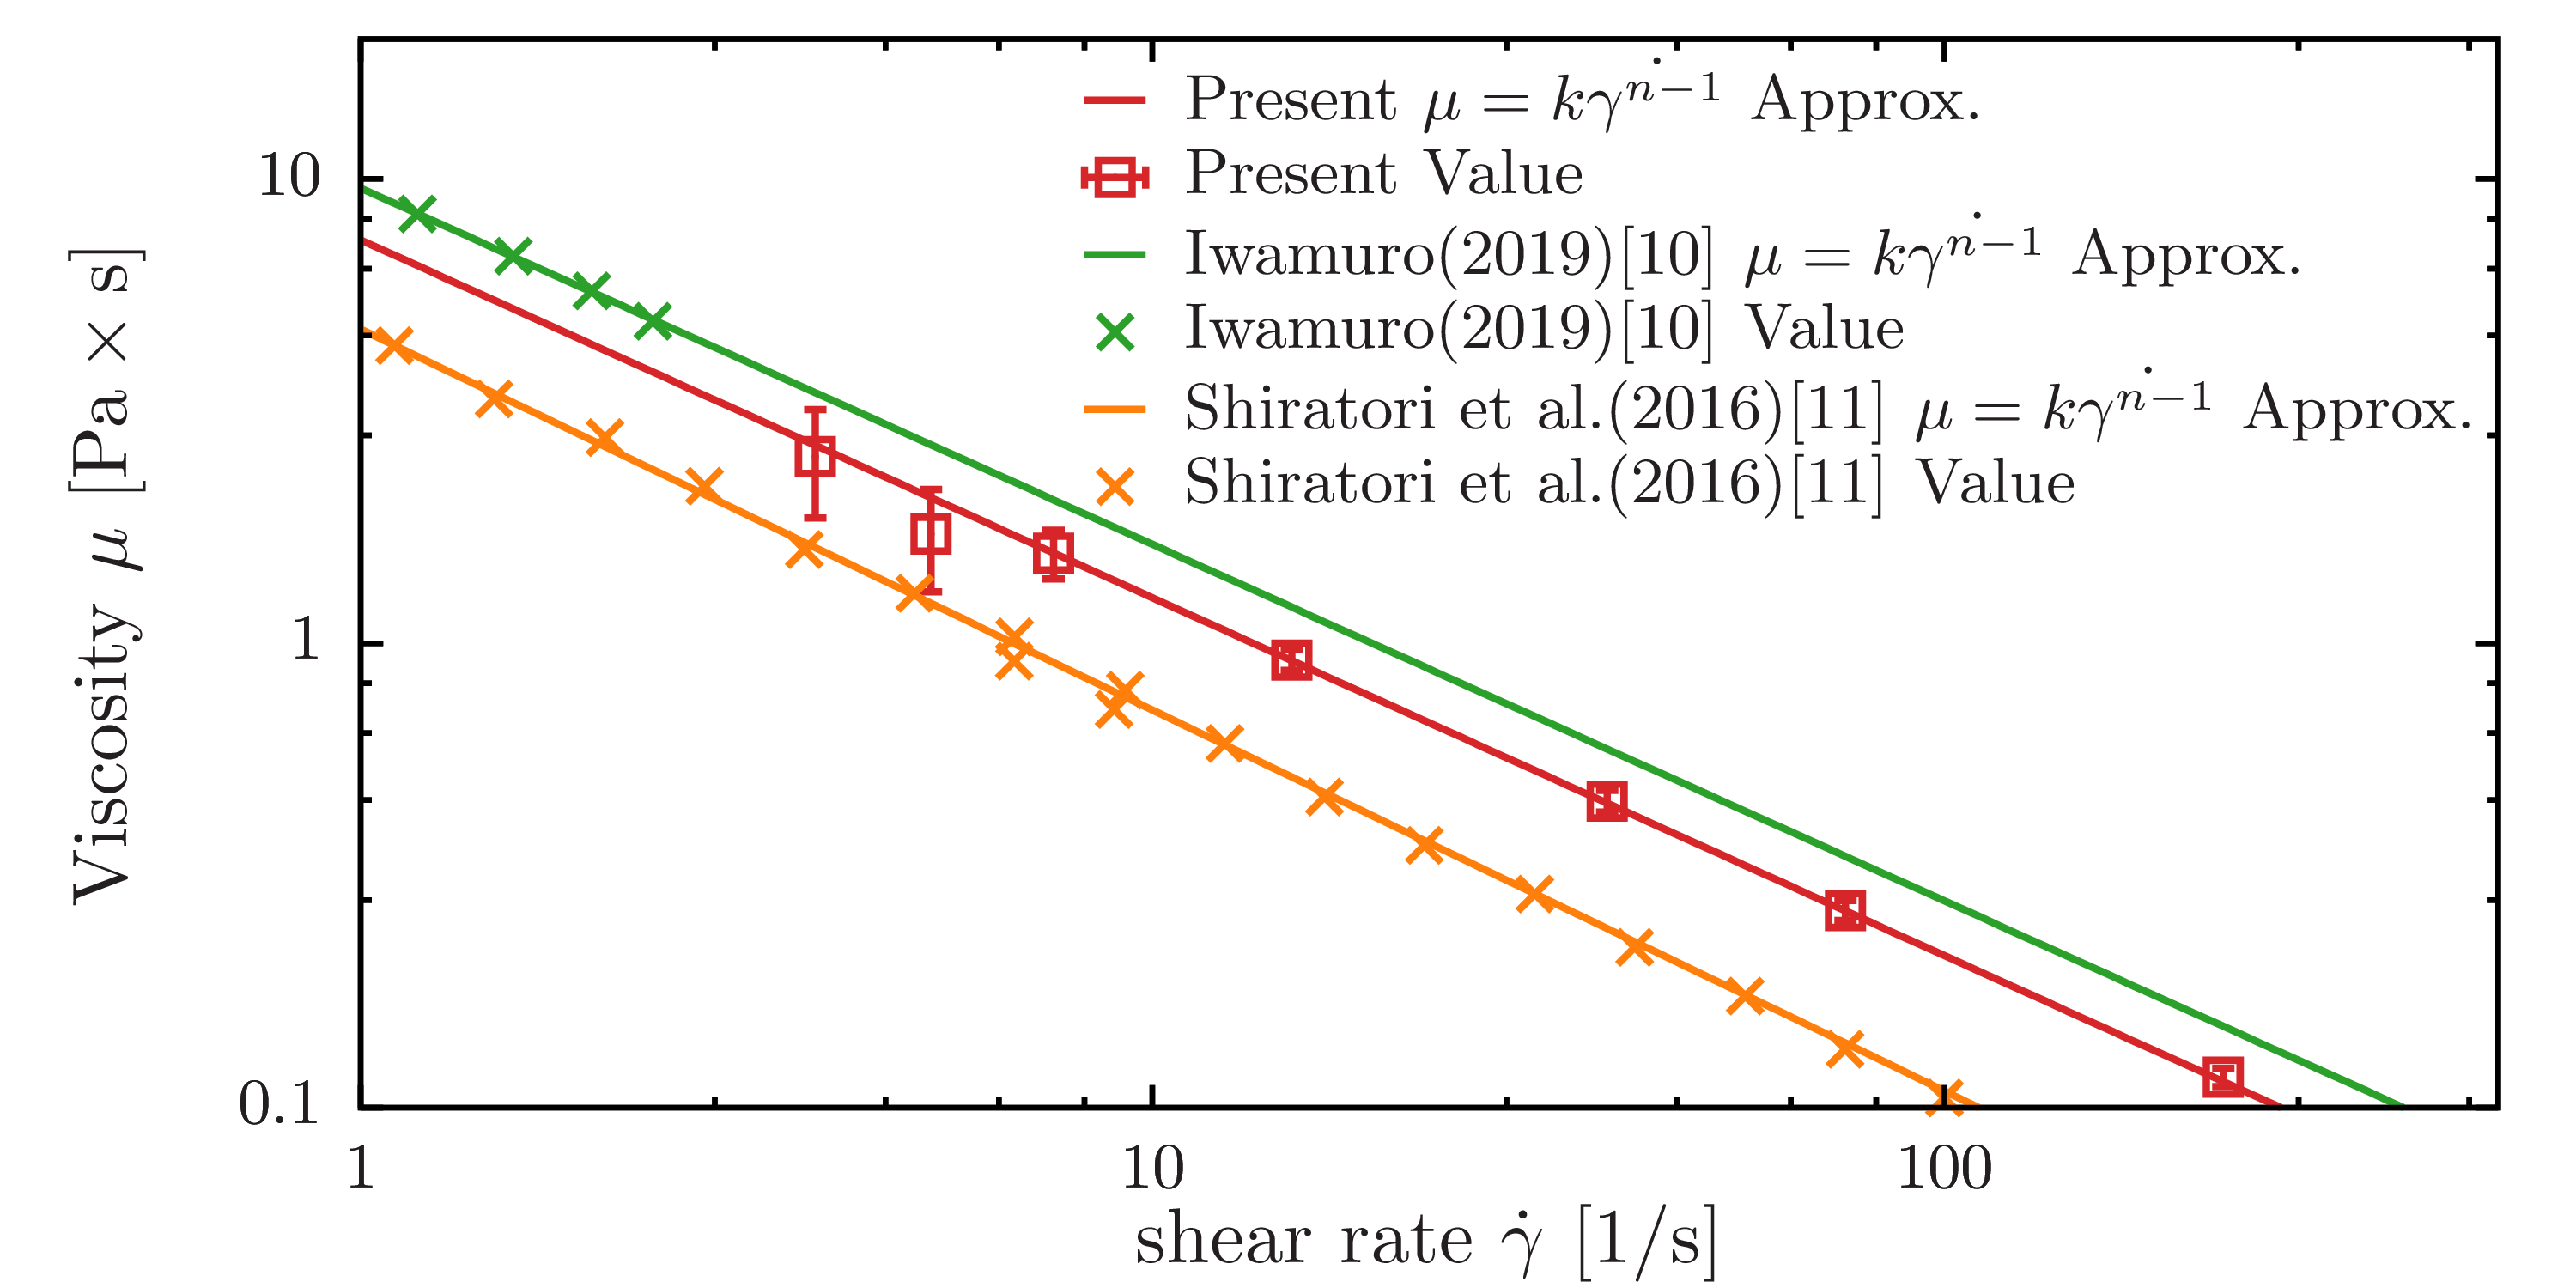
\includegraphics[width=12cm,clip]{4-Results/PAA-viscosity.png}
    \caption{Flow curve for 1wt.\%PAA solution.}
    \label{fig:PAA-vis}
\end{figure}

\newpage

\subsection{圧力場 計測結果}

0.5wt.\%PAA溶液における超音波圧力場の計測を行った結果をFig.\ref{fig:pressure}(a)に示す.また,1wt.\%PAA溶液における超音波圧力場の計測を行った結果をFig.\ref{fig:pressure}(b)に示す.縦軸は水槽底面からの高さ,横軸は圧力である.この結果を元にTable\ref{table:press}に圧力$P$の$y$方向平均値を示す.Iwamuro {\it et al.}\cite{ref:8}と比較して形成された圧力場が強いことが分かった.これは容器材質がIwamuro {\it et al.}\cite{ref:8}においてはガラス製であり,振動子板がSUS製であるが,今回どちらもアクリル製となっている.このことにより,超音波振動の伝達性能が向上したためだと考えられる.

\begin{table}[h]
    \centering
    \caption{Averaged value of pressure data.}
    \label{table:press}
    \begin{tabular}{c|c|c|c}\hline
                       & Present 0.5wt.\% PAA & Present 1wt.\% PAA & Iwamuro {\it et al.}\cite{ref:8} \\ \hline
        $\bar{P}$[kPa] & 97.3                 & 107.6              & 72                               \\ \hline
    \end{tabular}
\end{table}

\begin{figure}[ht]
    \centering
    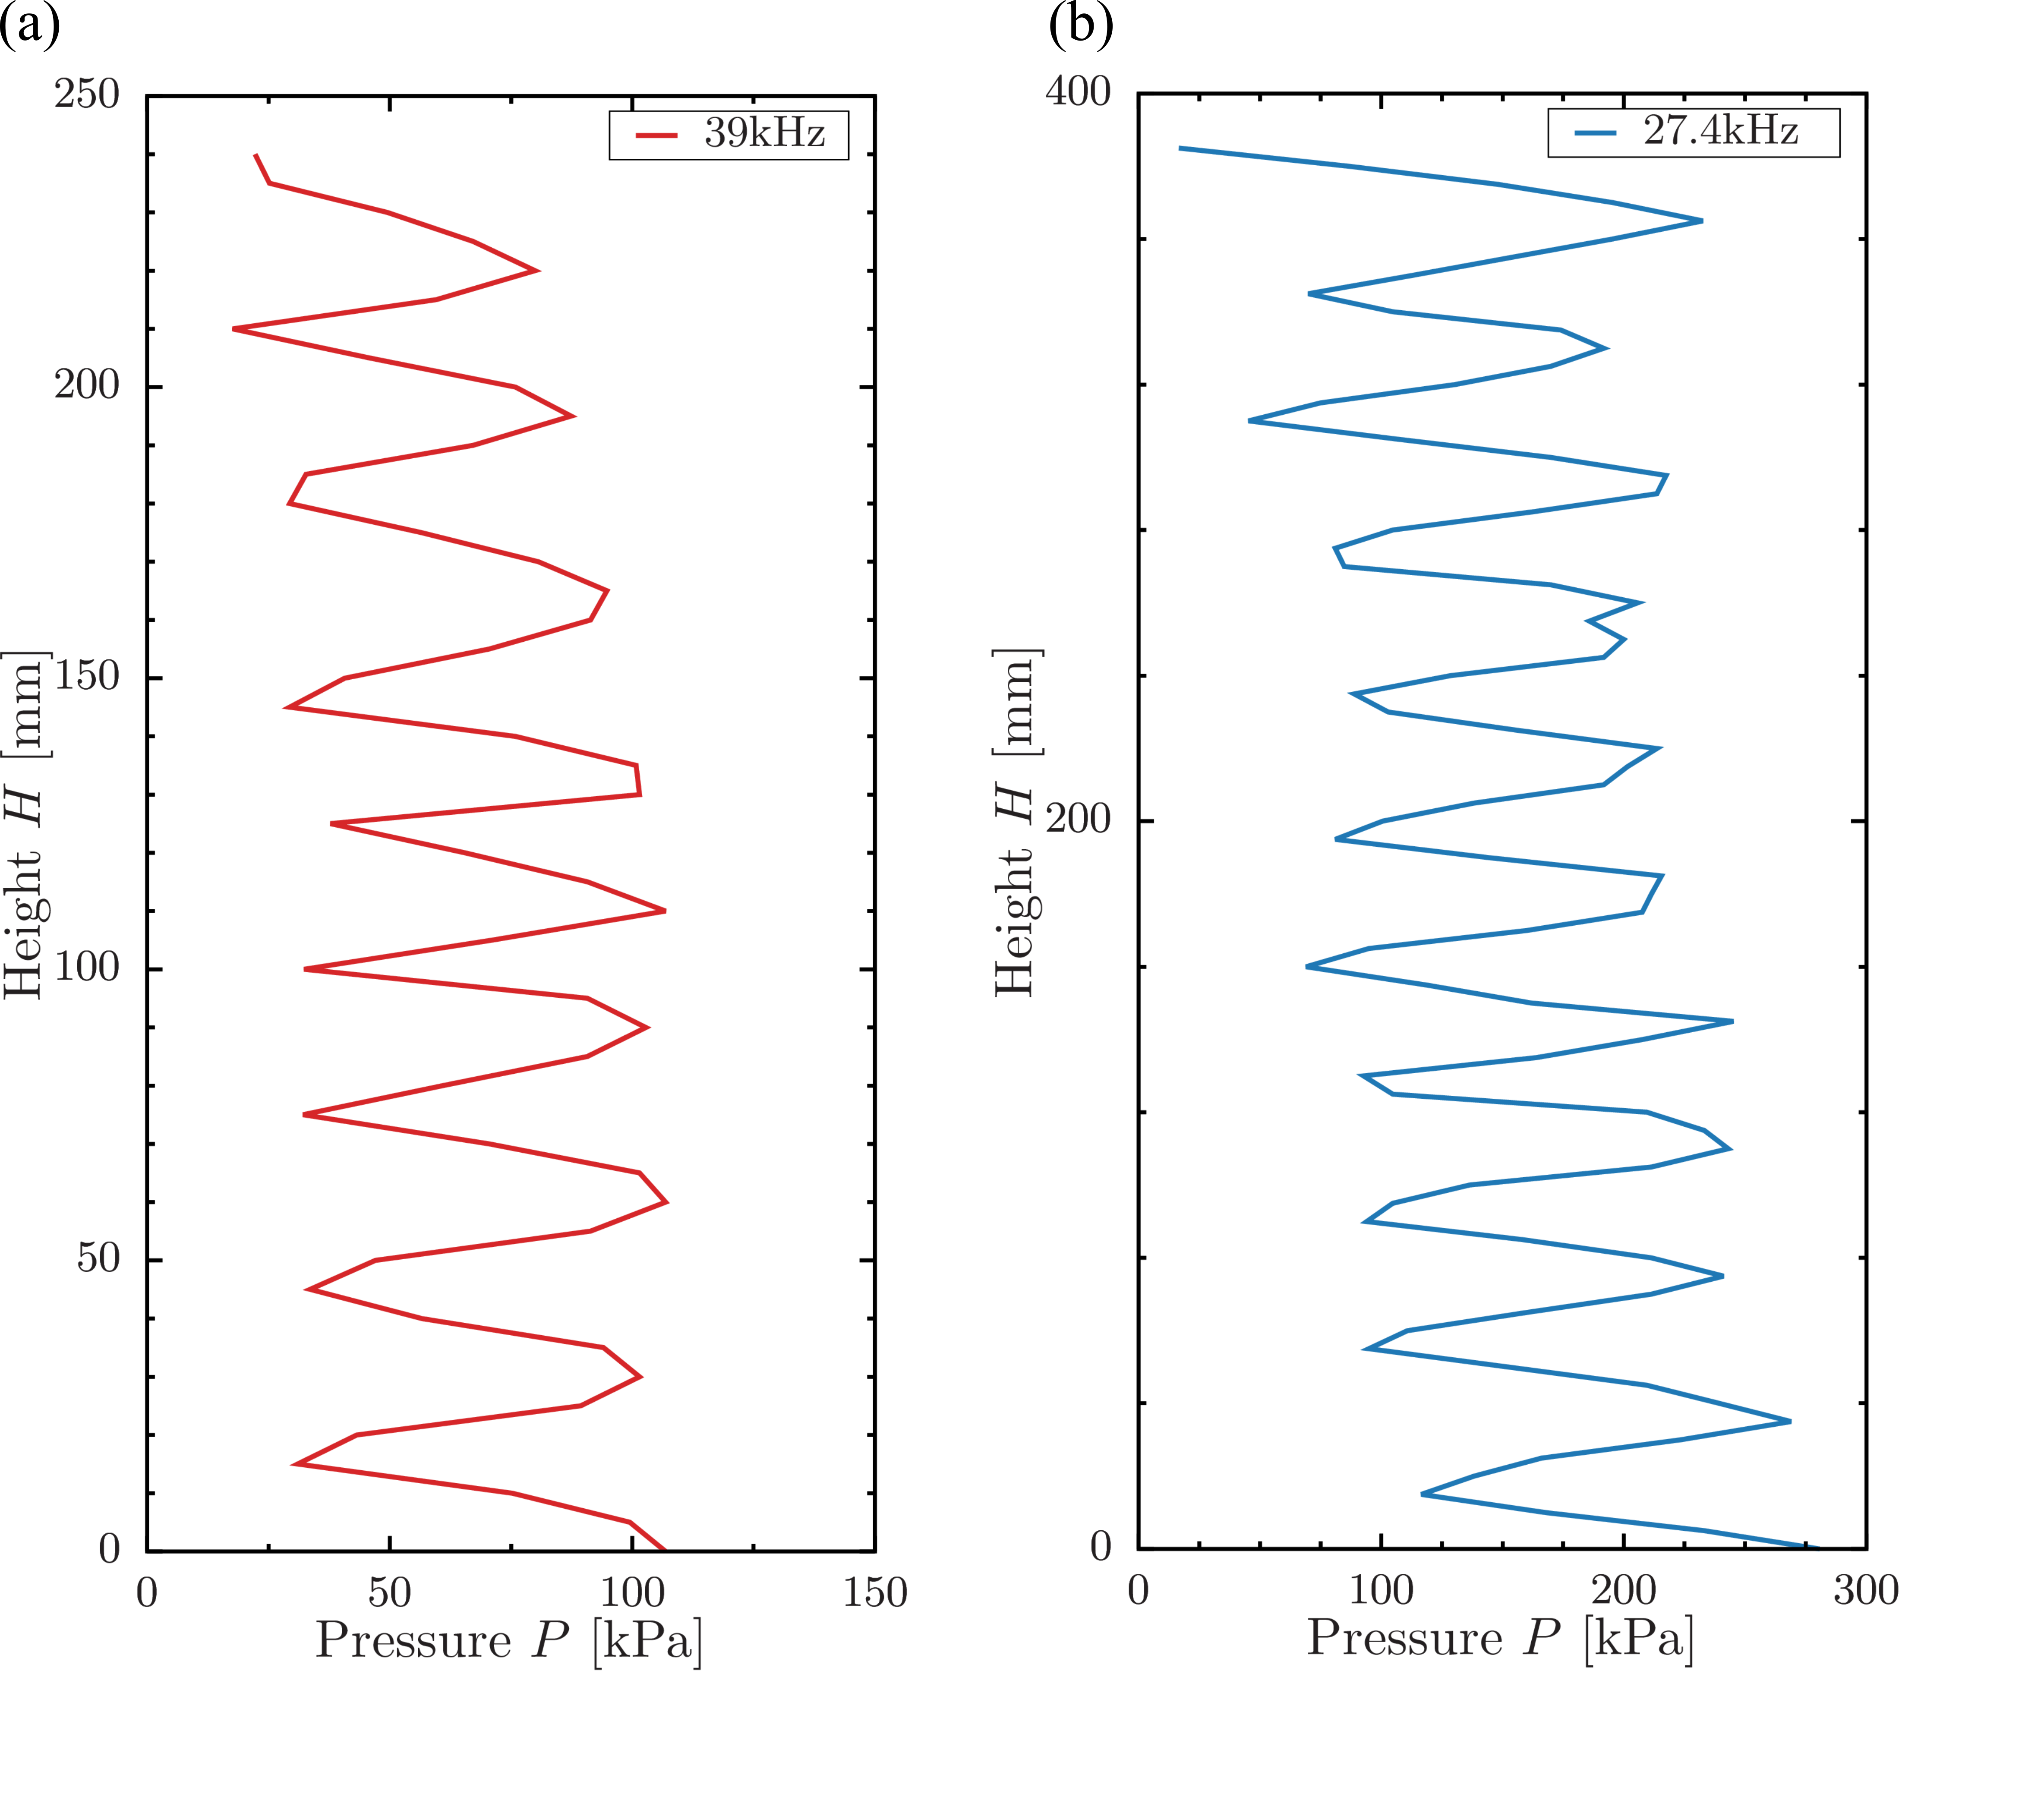
\includegraphics[width=9.5cm,clip]{4-Results/press.png}
    \caption{Pressure field in PAA solution measurement results.}
    \label{fig:pressure}
\end{figure}

\newpage

\subsection{落下球 実験結果}

\subsubsection{水道水}

水道水中における球の落下速度を解析した結果をFig.\ref{fig:water}に示す.縦軸は落下速度,横軸は落下開始時からの経過時間である.図より,水道水中において超音波照射の有無による球の落下速度の変化は発生しなかった.

\begin{figure}[ht]
    \centering
    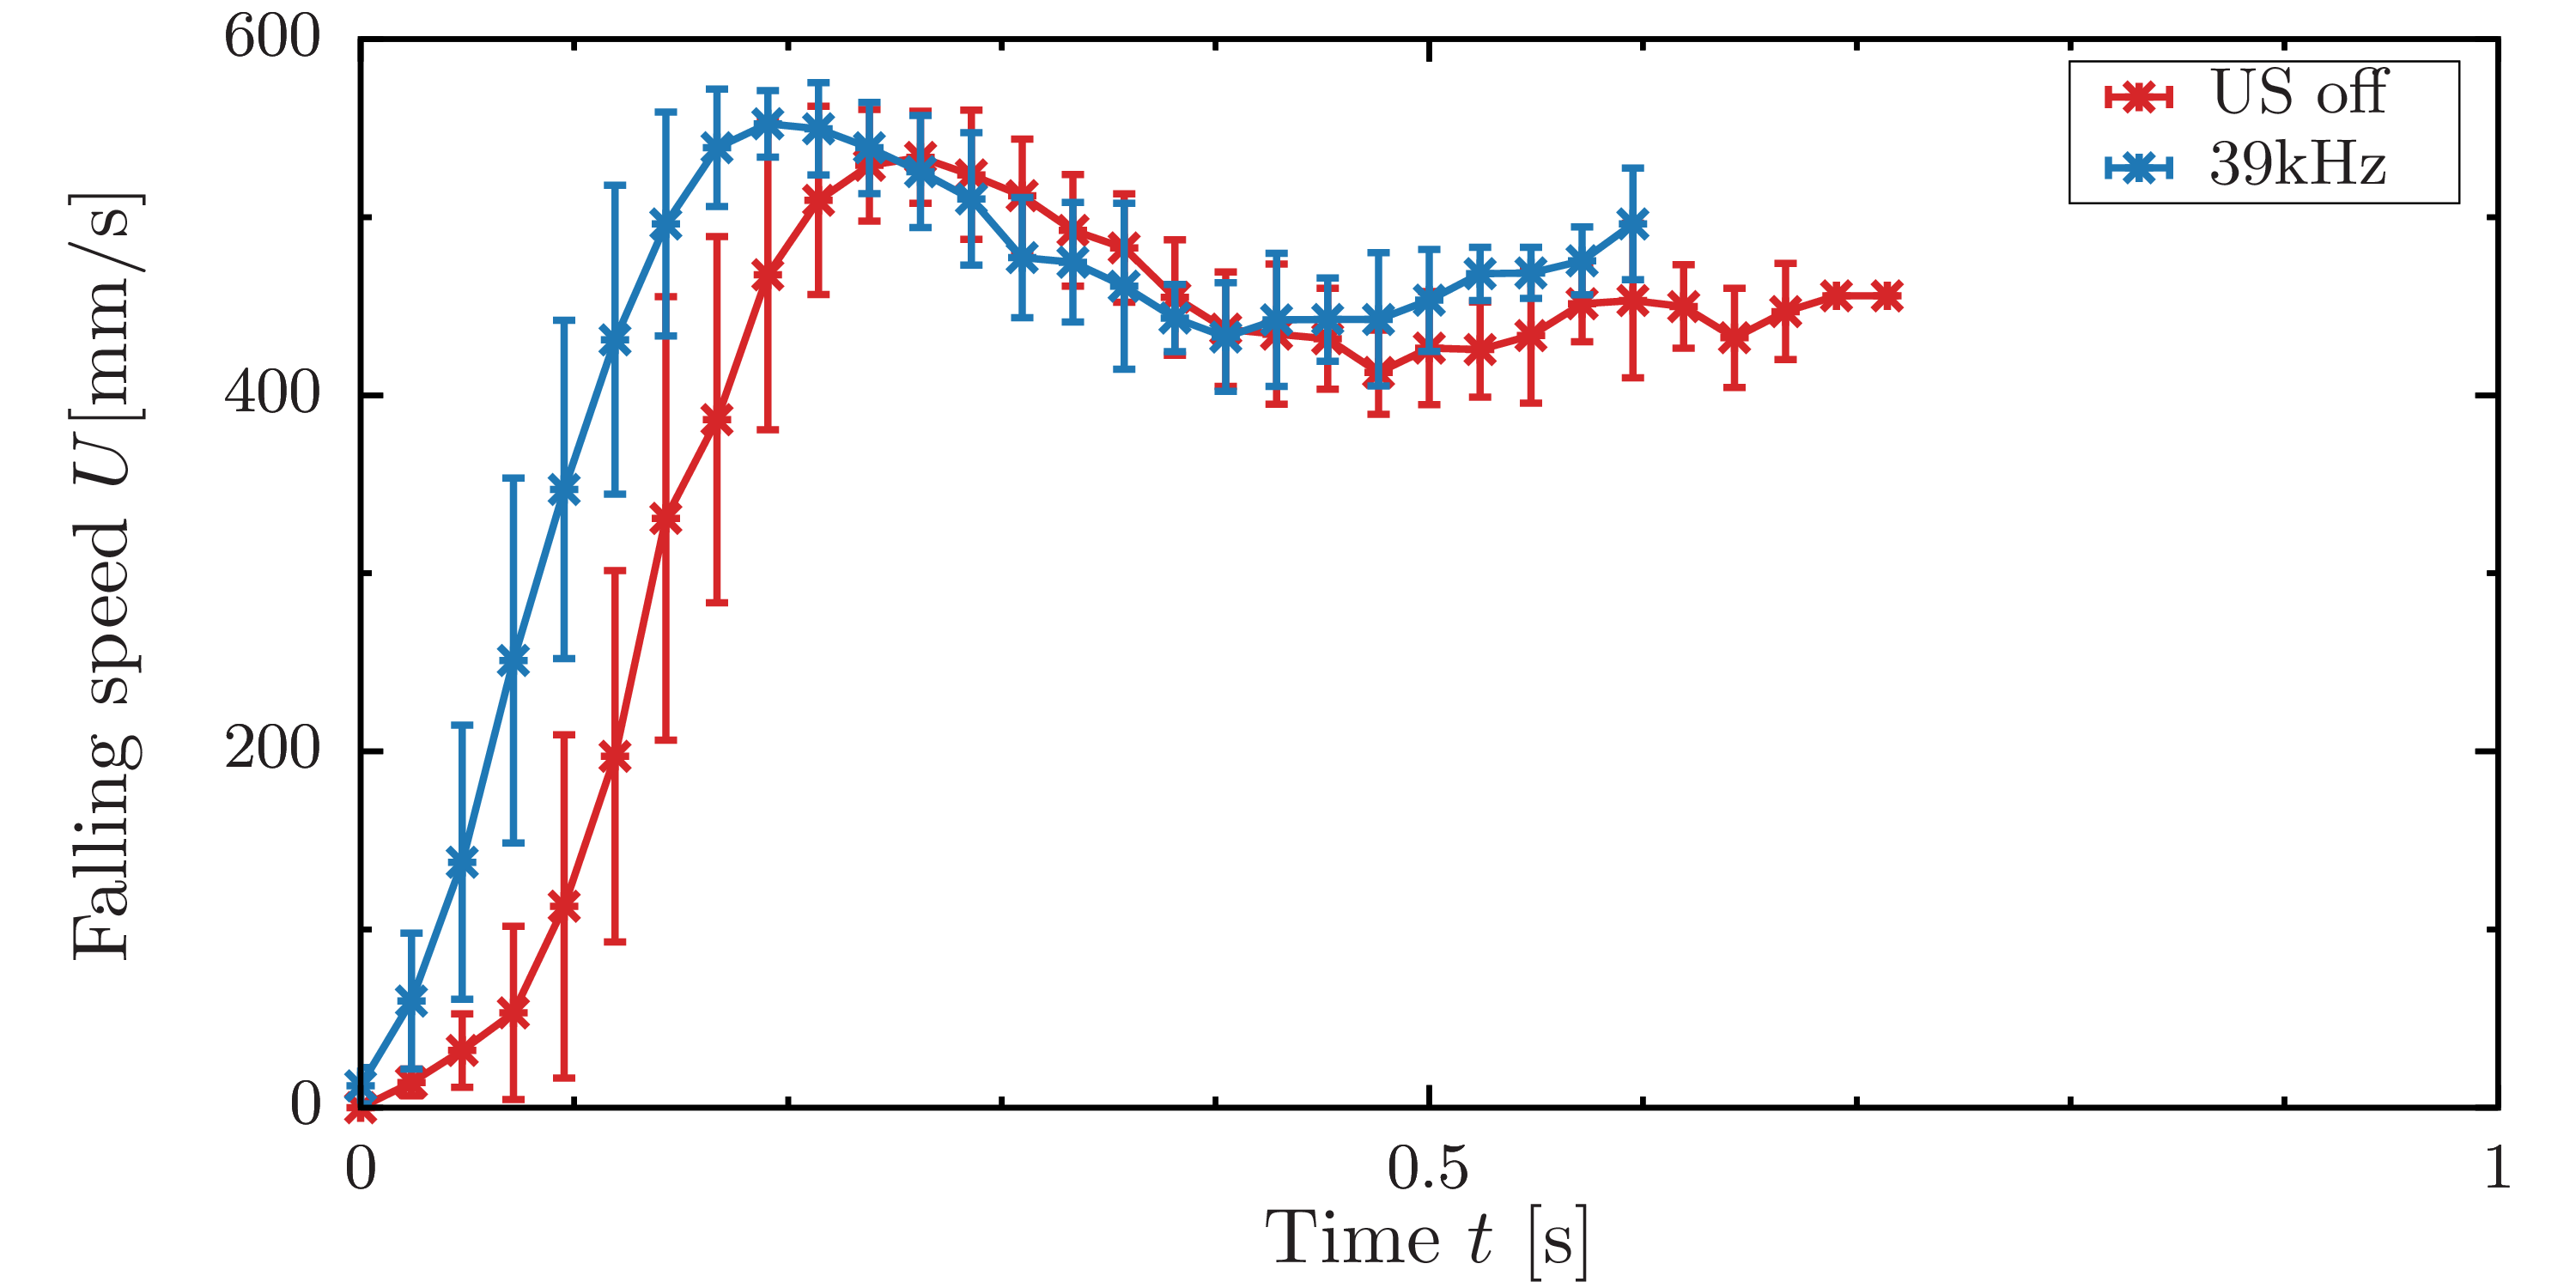
\includegraphics[width=11cm,clip]{./4-Results/f-water.png}
    \caption{Velocity of a falling sphere with a diameter of 2.4mm in water with or without ultrasound irradiation.}
    \label{fig:water}
\end{figure}

\subsubsection{0.5wt.\%PAA溶液}

0.5wt.\%PAA溶液中における球の落下速度を解析した結果をFig.\ref{fig:0.5PAA-falling}に示す.縦軸は落下速度,横軸は落下開始時からの経過時間である.超音波圧力場振動によって弱い高速化効果が見られる.

超音波照射なしの状態における1から5試行目の結果をFig.\ref{fig:0.5PAA-falling1-5}に,6から10試行目の結果をFig.\ref{fig:0.5PAA-falling6-10}に示す.試行回数を経るごとに球の落下速度が大きくなっていることが分かる.これは履歴効果により,球の落下による影響が発生しているためであると思われる.同様に,超音波照射ありの状態における1から5試行目の結果をFig.\ref{fig:0.5onPAA-falling1-5}に,6から10試行目の結果をFig.\ref{fig:0.5onPAA-falling6-10}に示す.先述の超音波なしの状態と同様に試行回数を経るごとに球の落下速度が大きくなっていることが分かった.

\begin{figure}[ht]
    \centering
    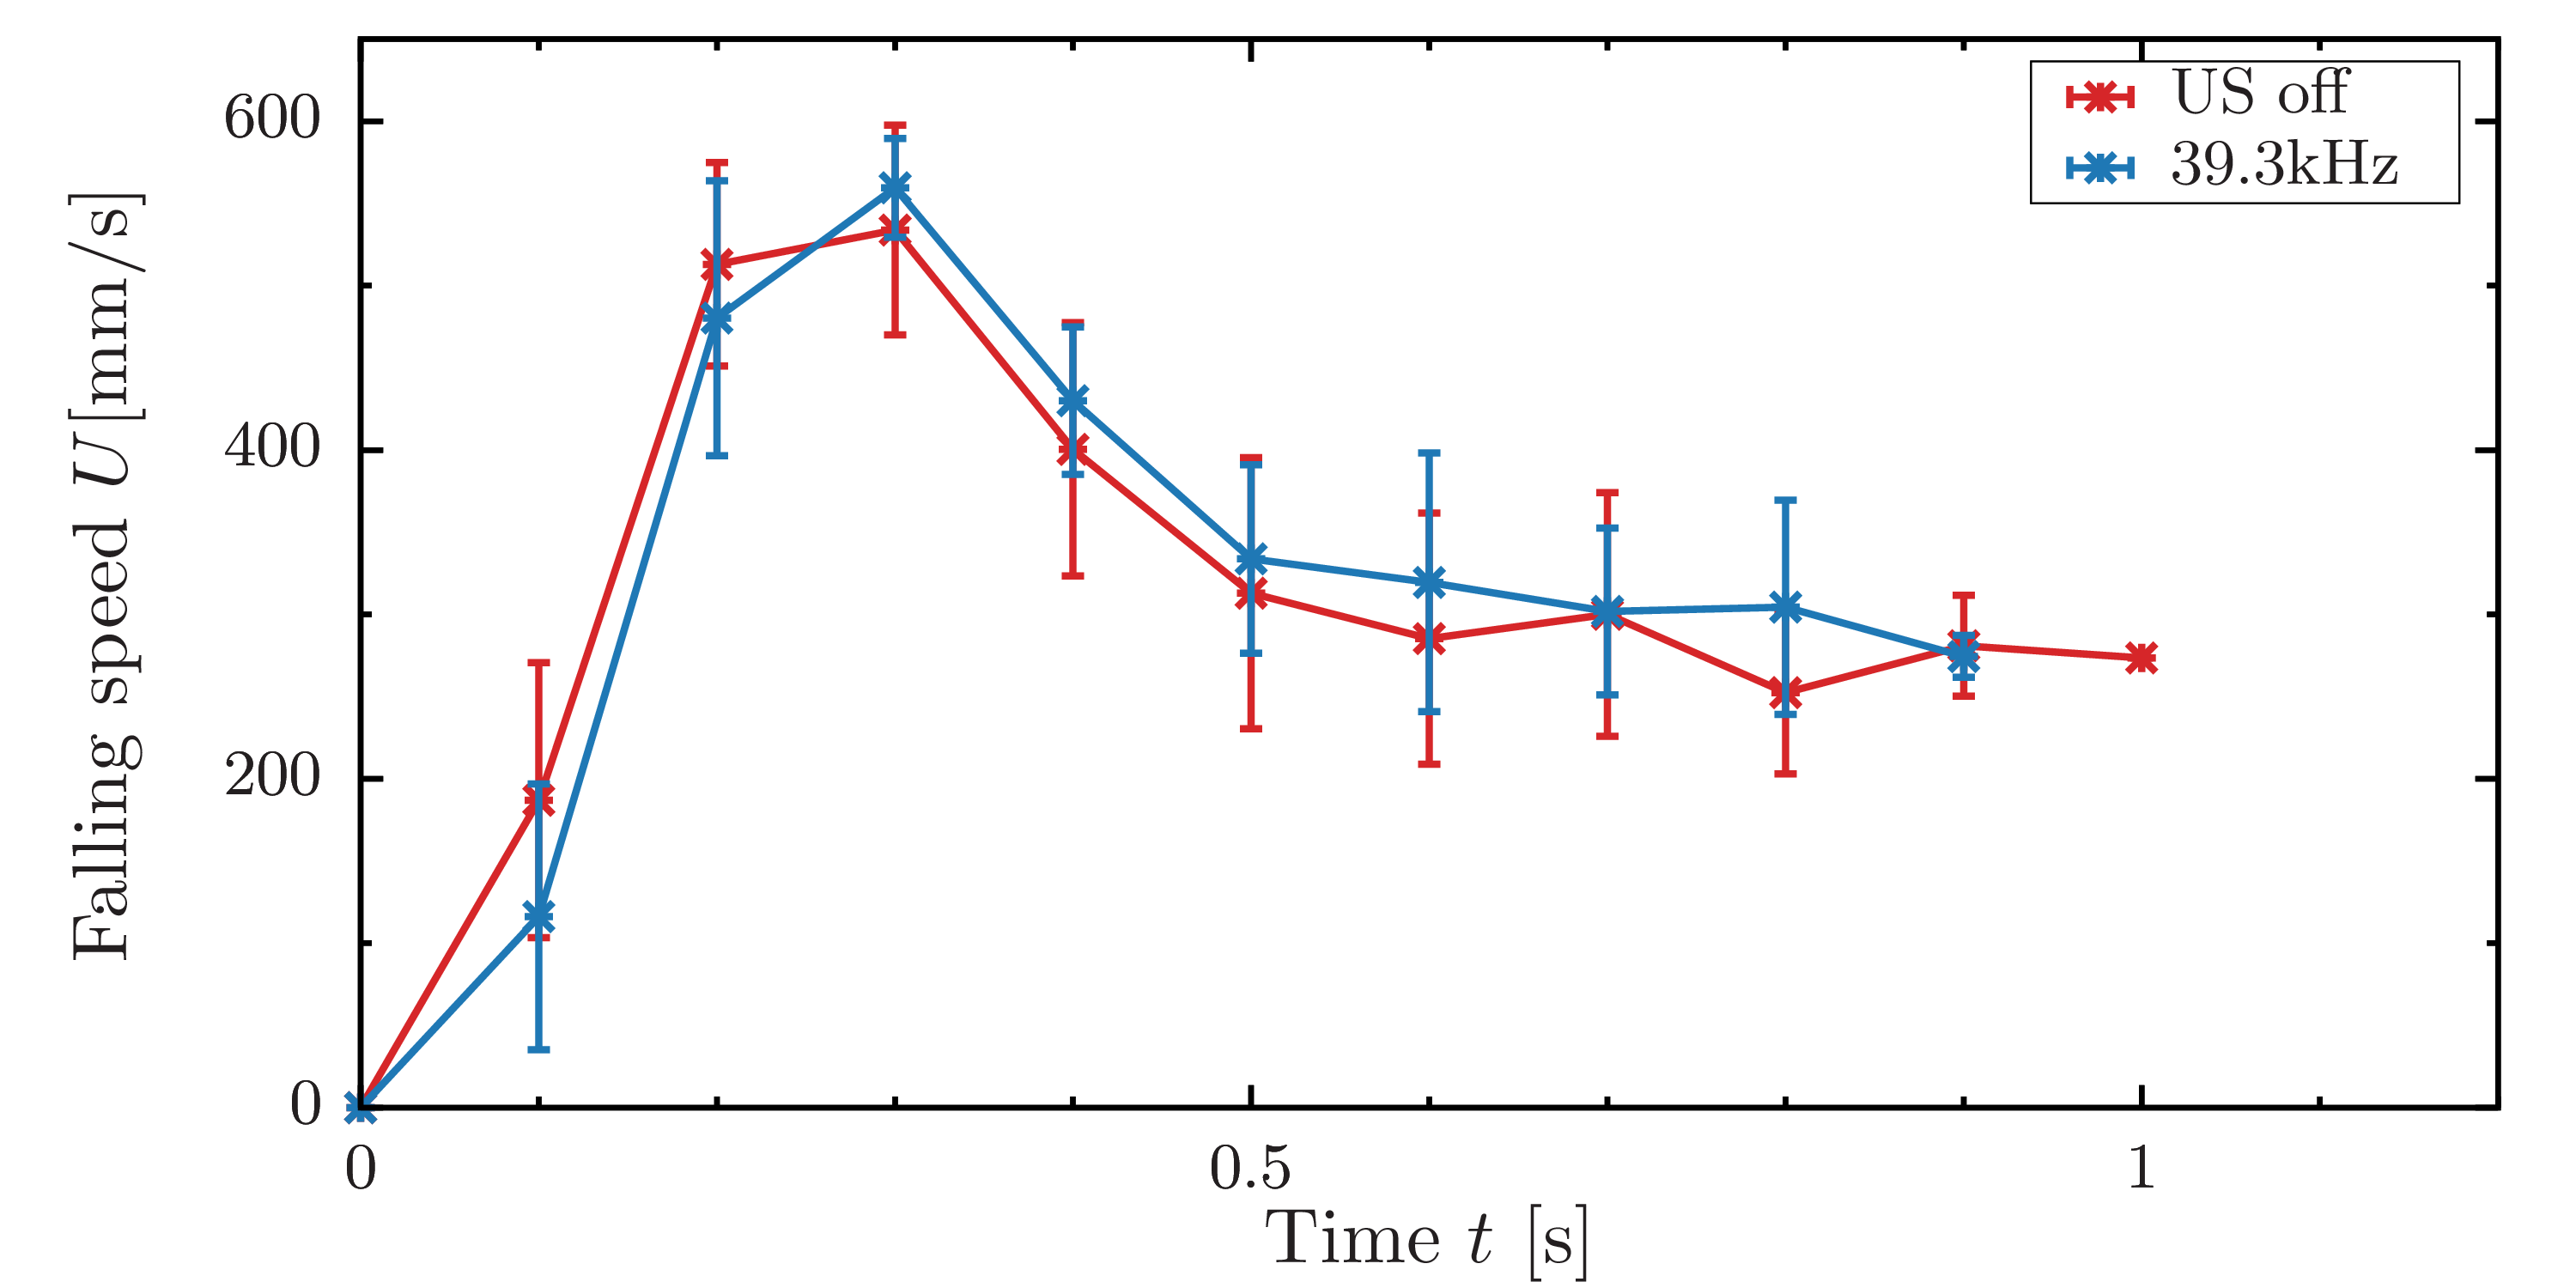
\includegraphics[width=12cm,clip]{./4-Results/s0.5.png}
    \caption{Falling velocity of a sphere in 0.5wt.\%PAA solution with and without ultrasound irradiation.}
    \label{fig:0.5PAA-falling}
    \centering
    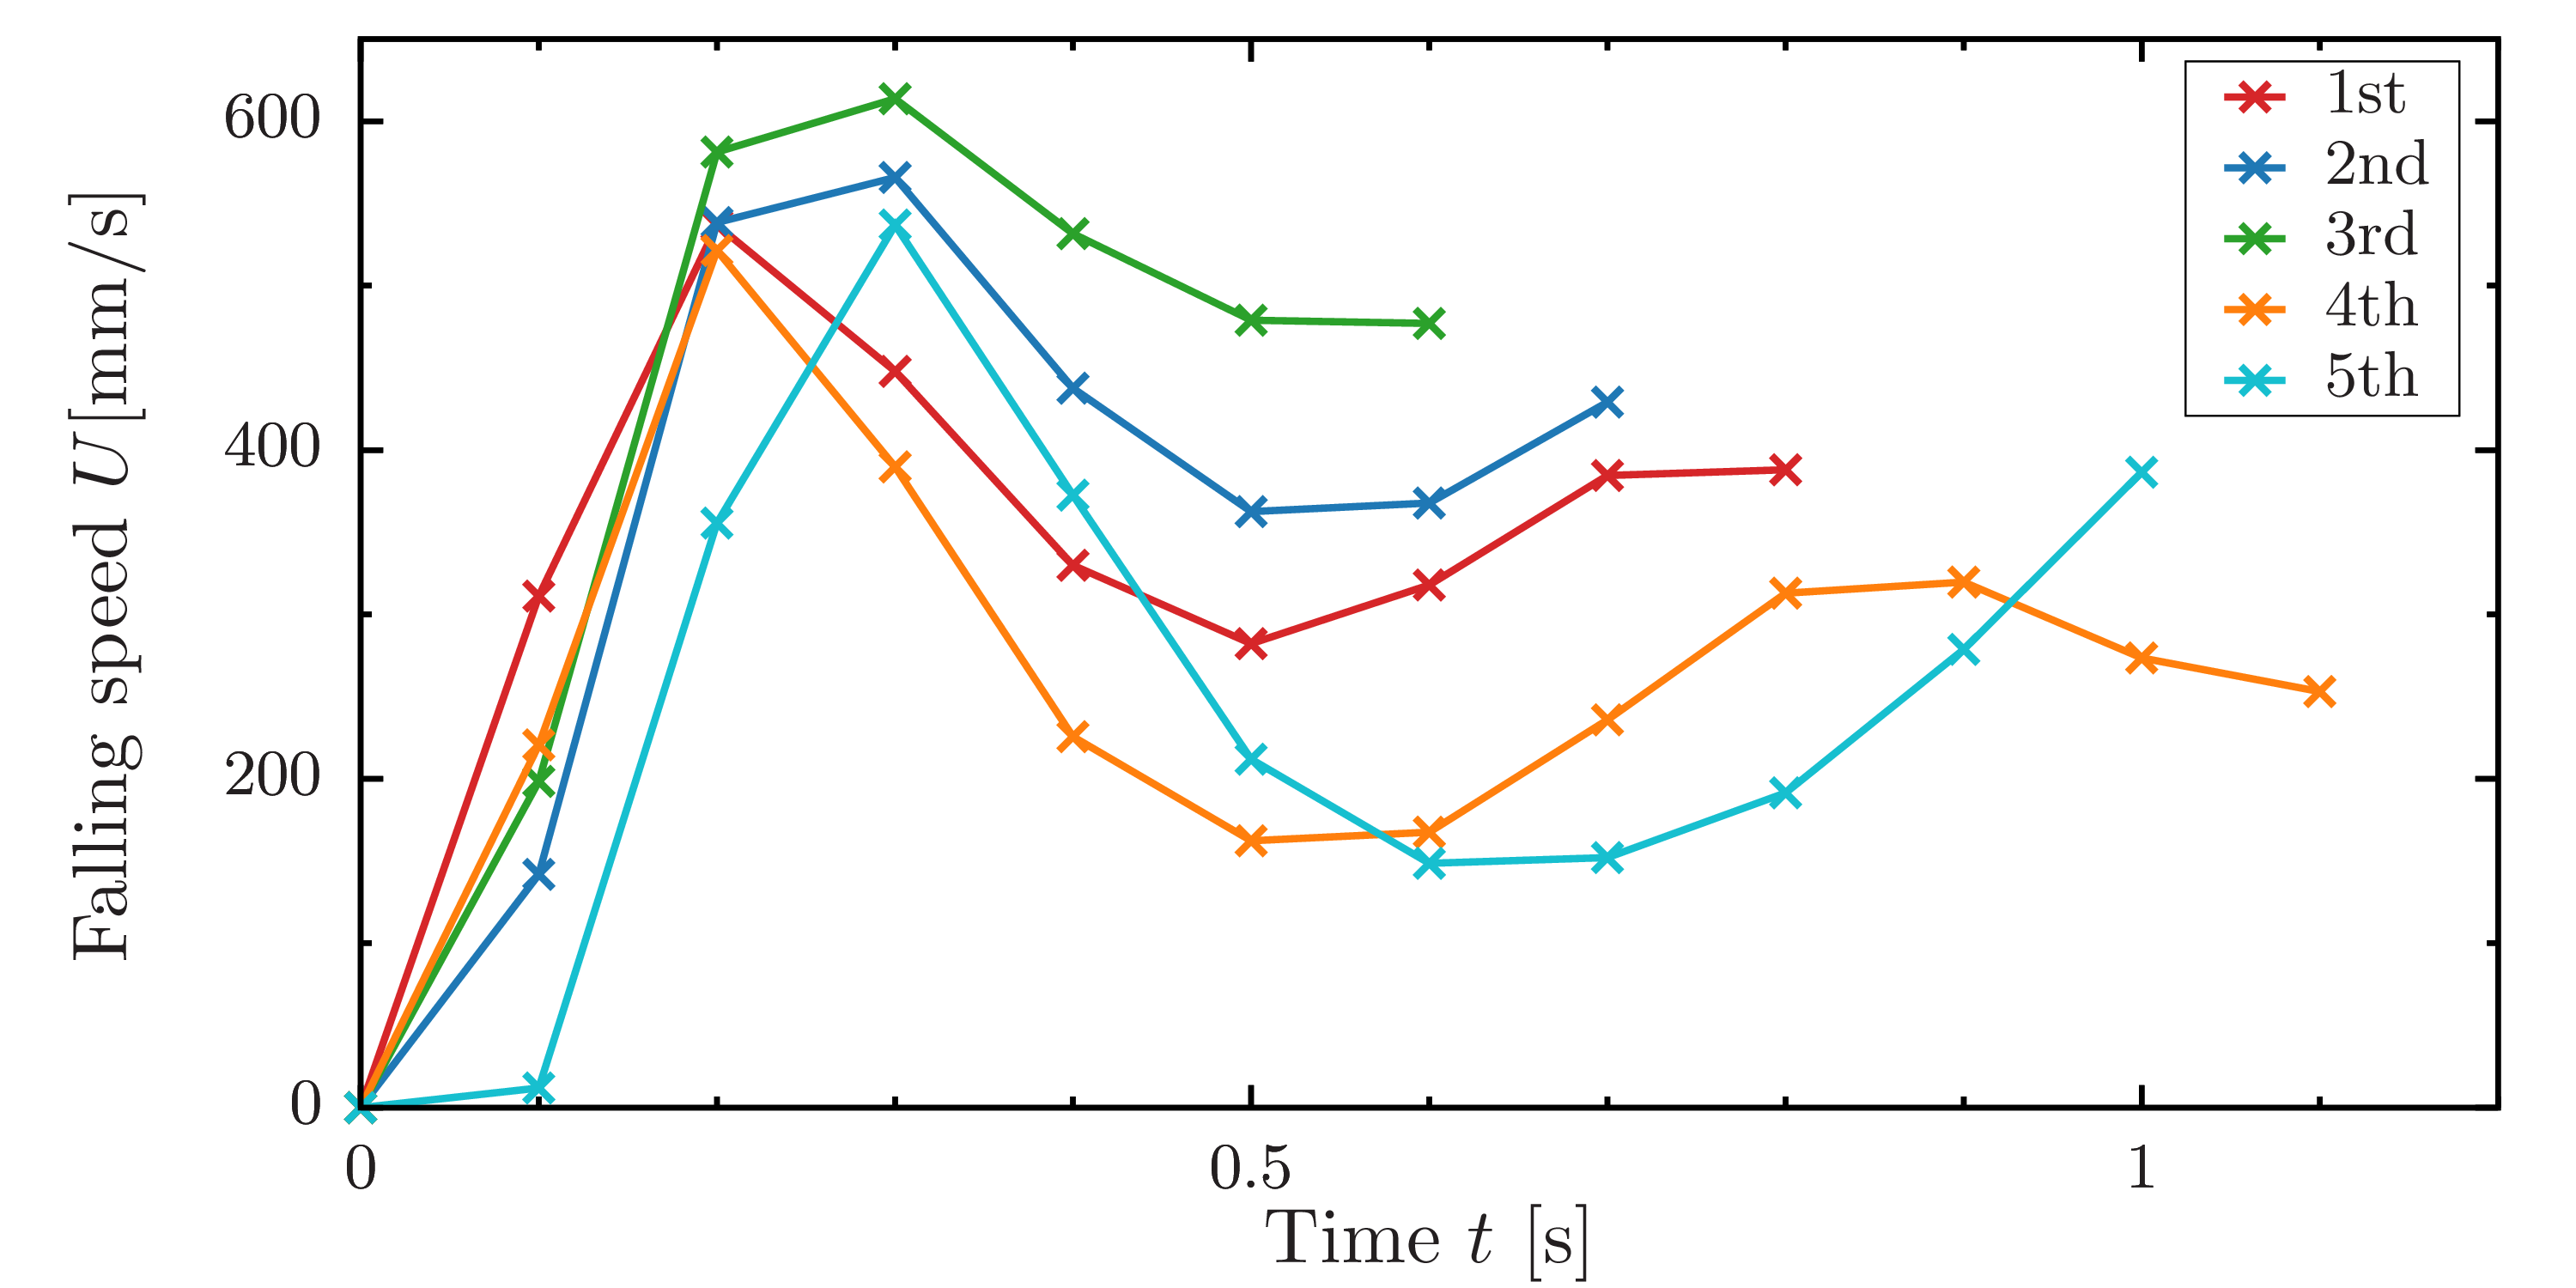
\includegraphics[width=12cm,clip]{4-Results/s0.5-0-1-5.png}
    \caption{Falling velocity of the sphere for each trial (\#1 to \#5) in 0.5wt.\%PAA solution without ultrasonic irradiation.}
    \label{fig:0.5PAA-falling1-5}
\end{figure}
\begin{figure}[ht]
    \centering
    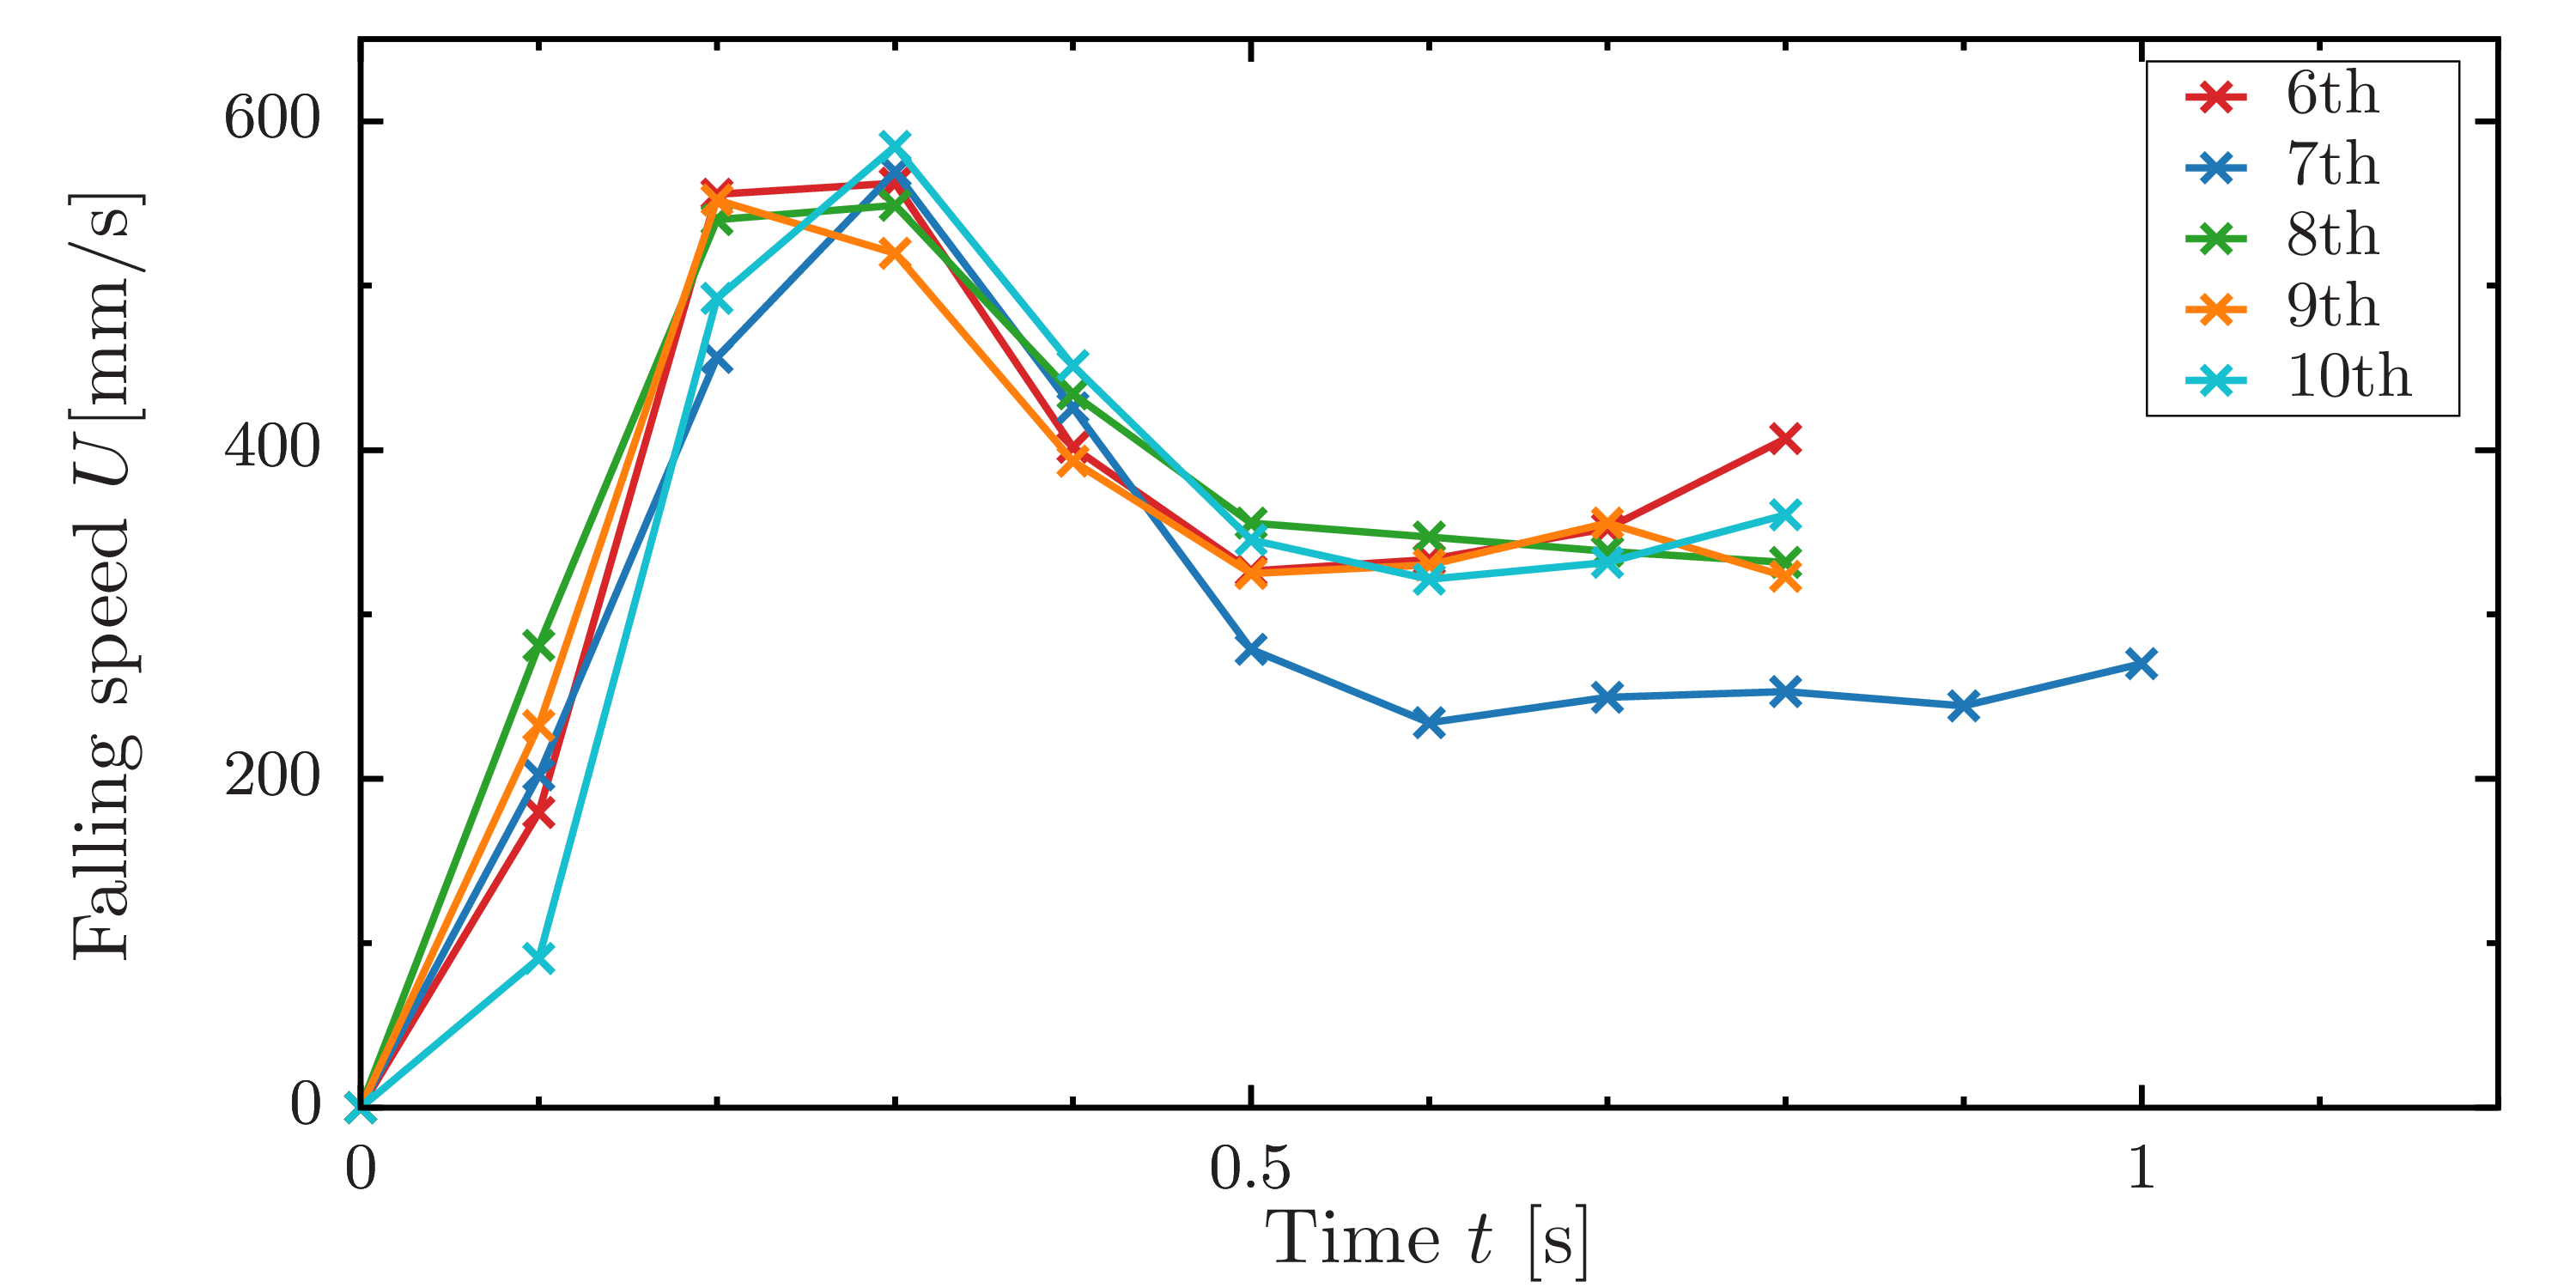
\includegraphics[width=12cm,clip]{4-Results/s0.5-0-6-10.png}
    \caption{Falling velocity of the sphere for each trial (\#6 to \#10) in 0.5wt.\%PAA solution without ultrasonic irradiation.}
    \label{fig:0.5PAA-falling6-10}
    \centering
    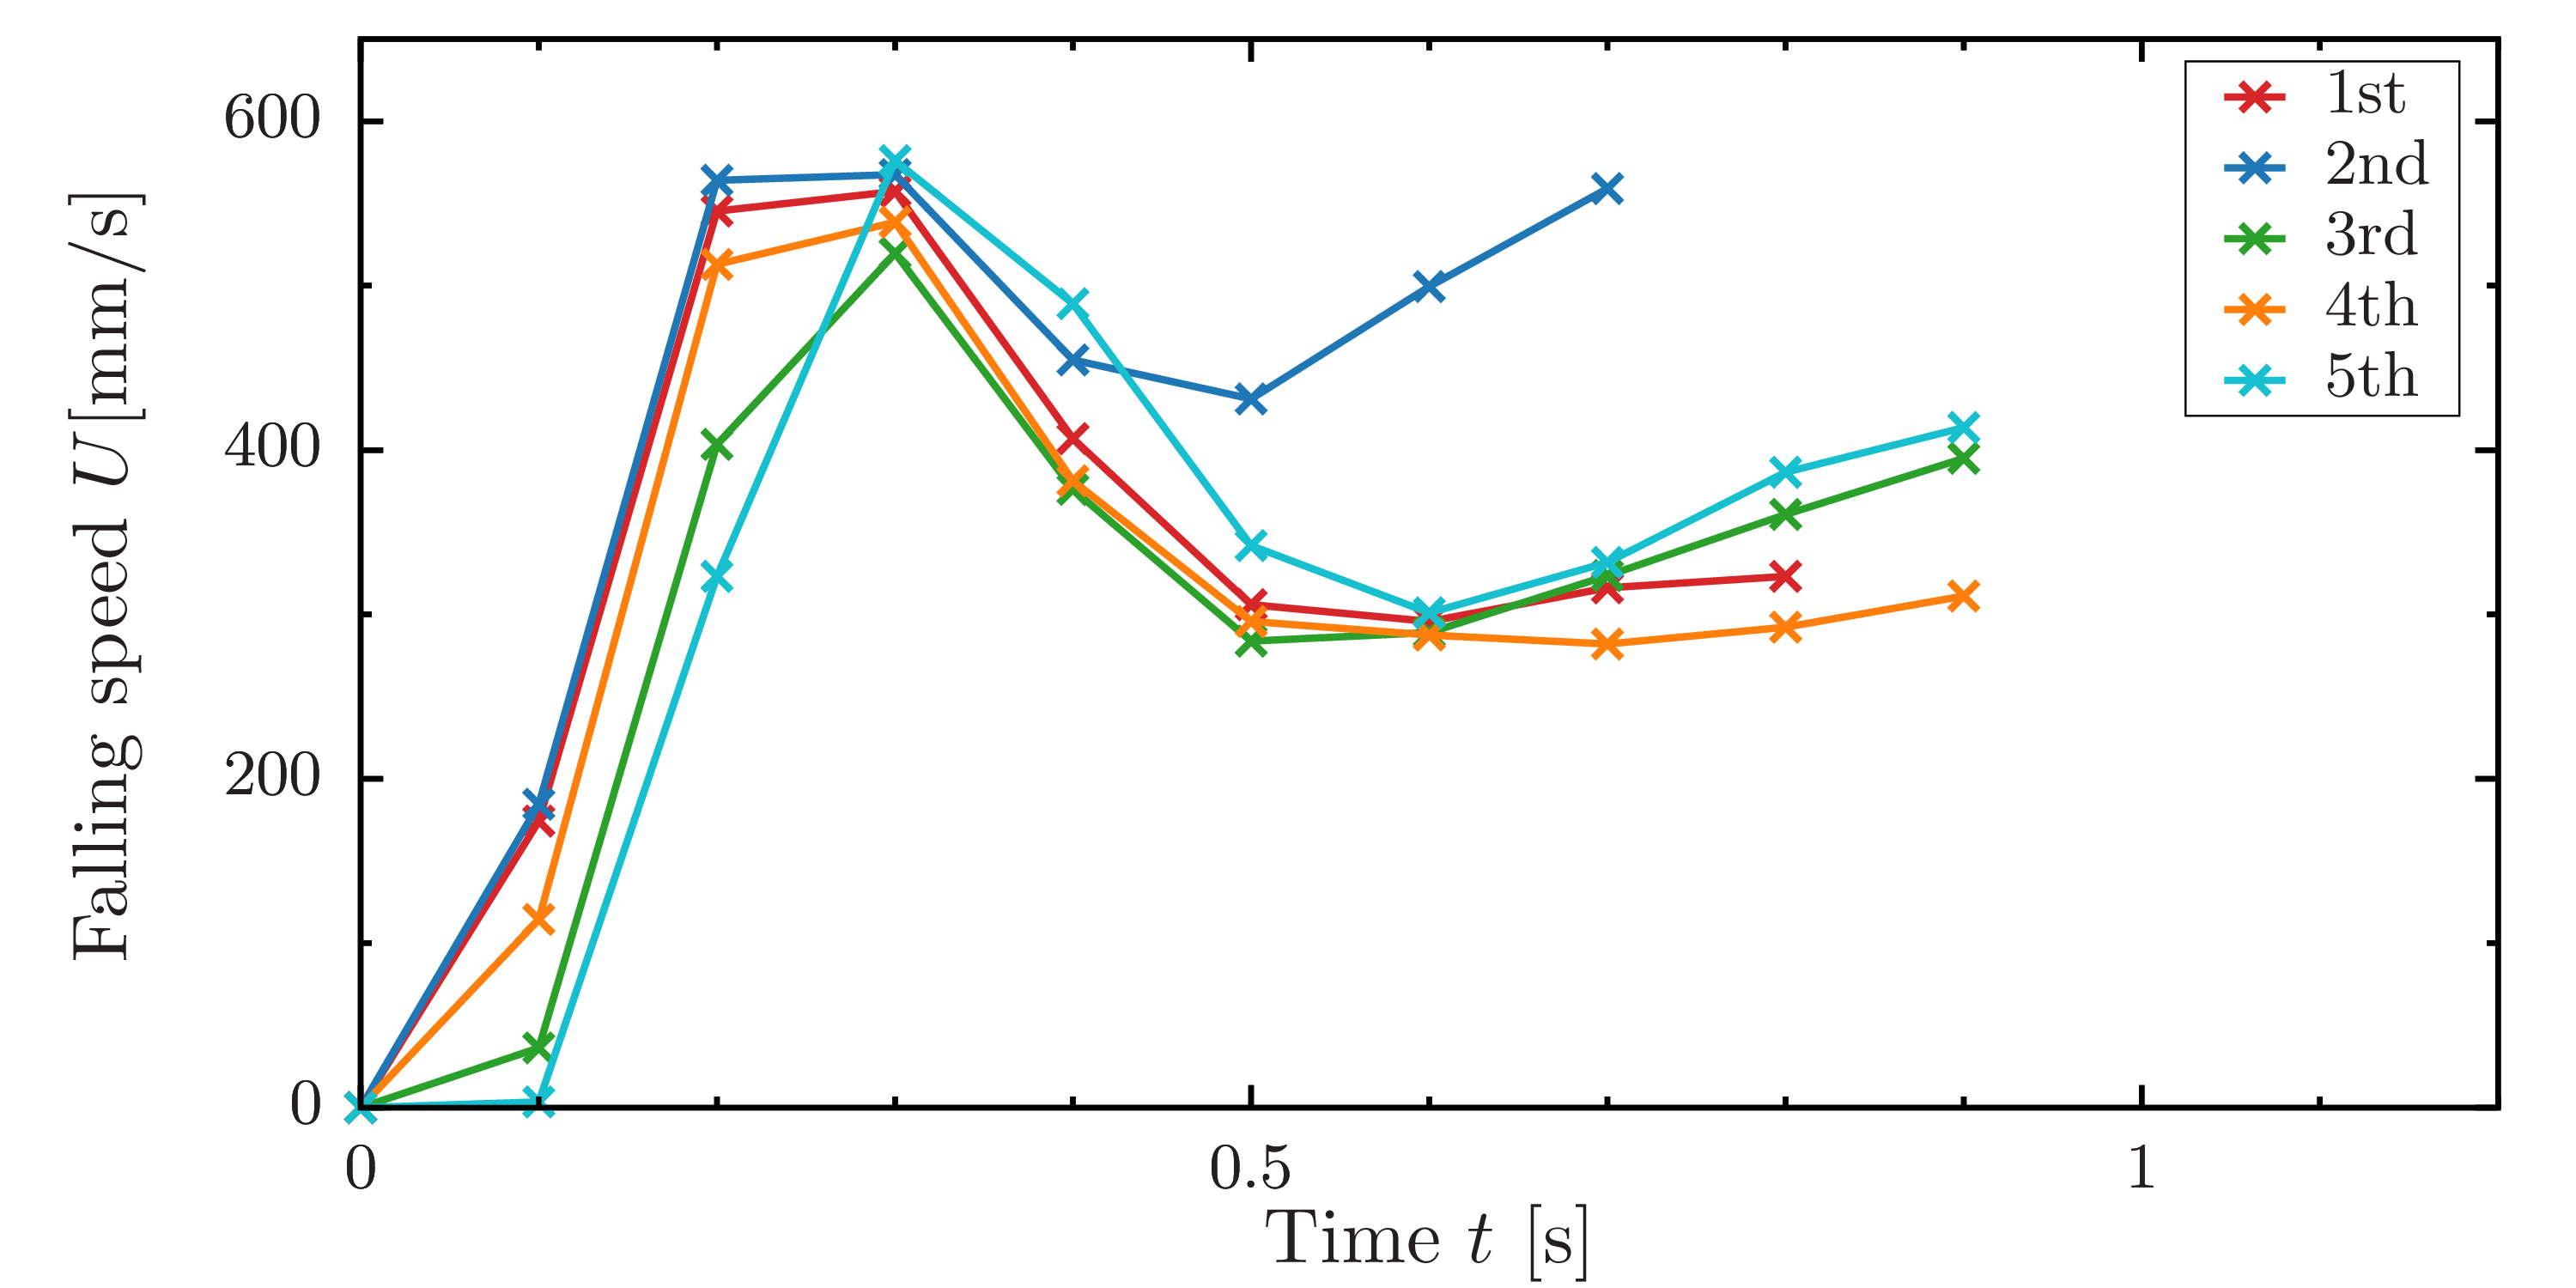
\includegraphics[width=12cm,clip]{4-Results/s0.5-39-1-5.png}
    \caption{Falling velocity of the sphere for each trial (\#1 to \#5) in 0.5wt.\%PAA solution with ultrasonic irradiation.}
    \label{fig:0.5onPAA-falling1-5}
    \centering
    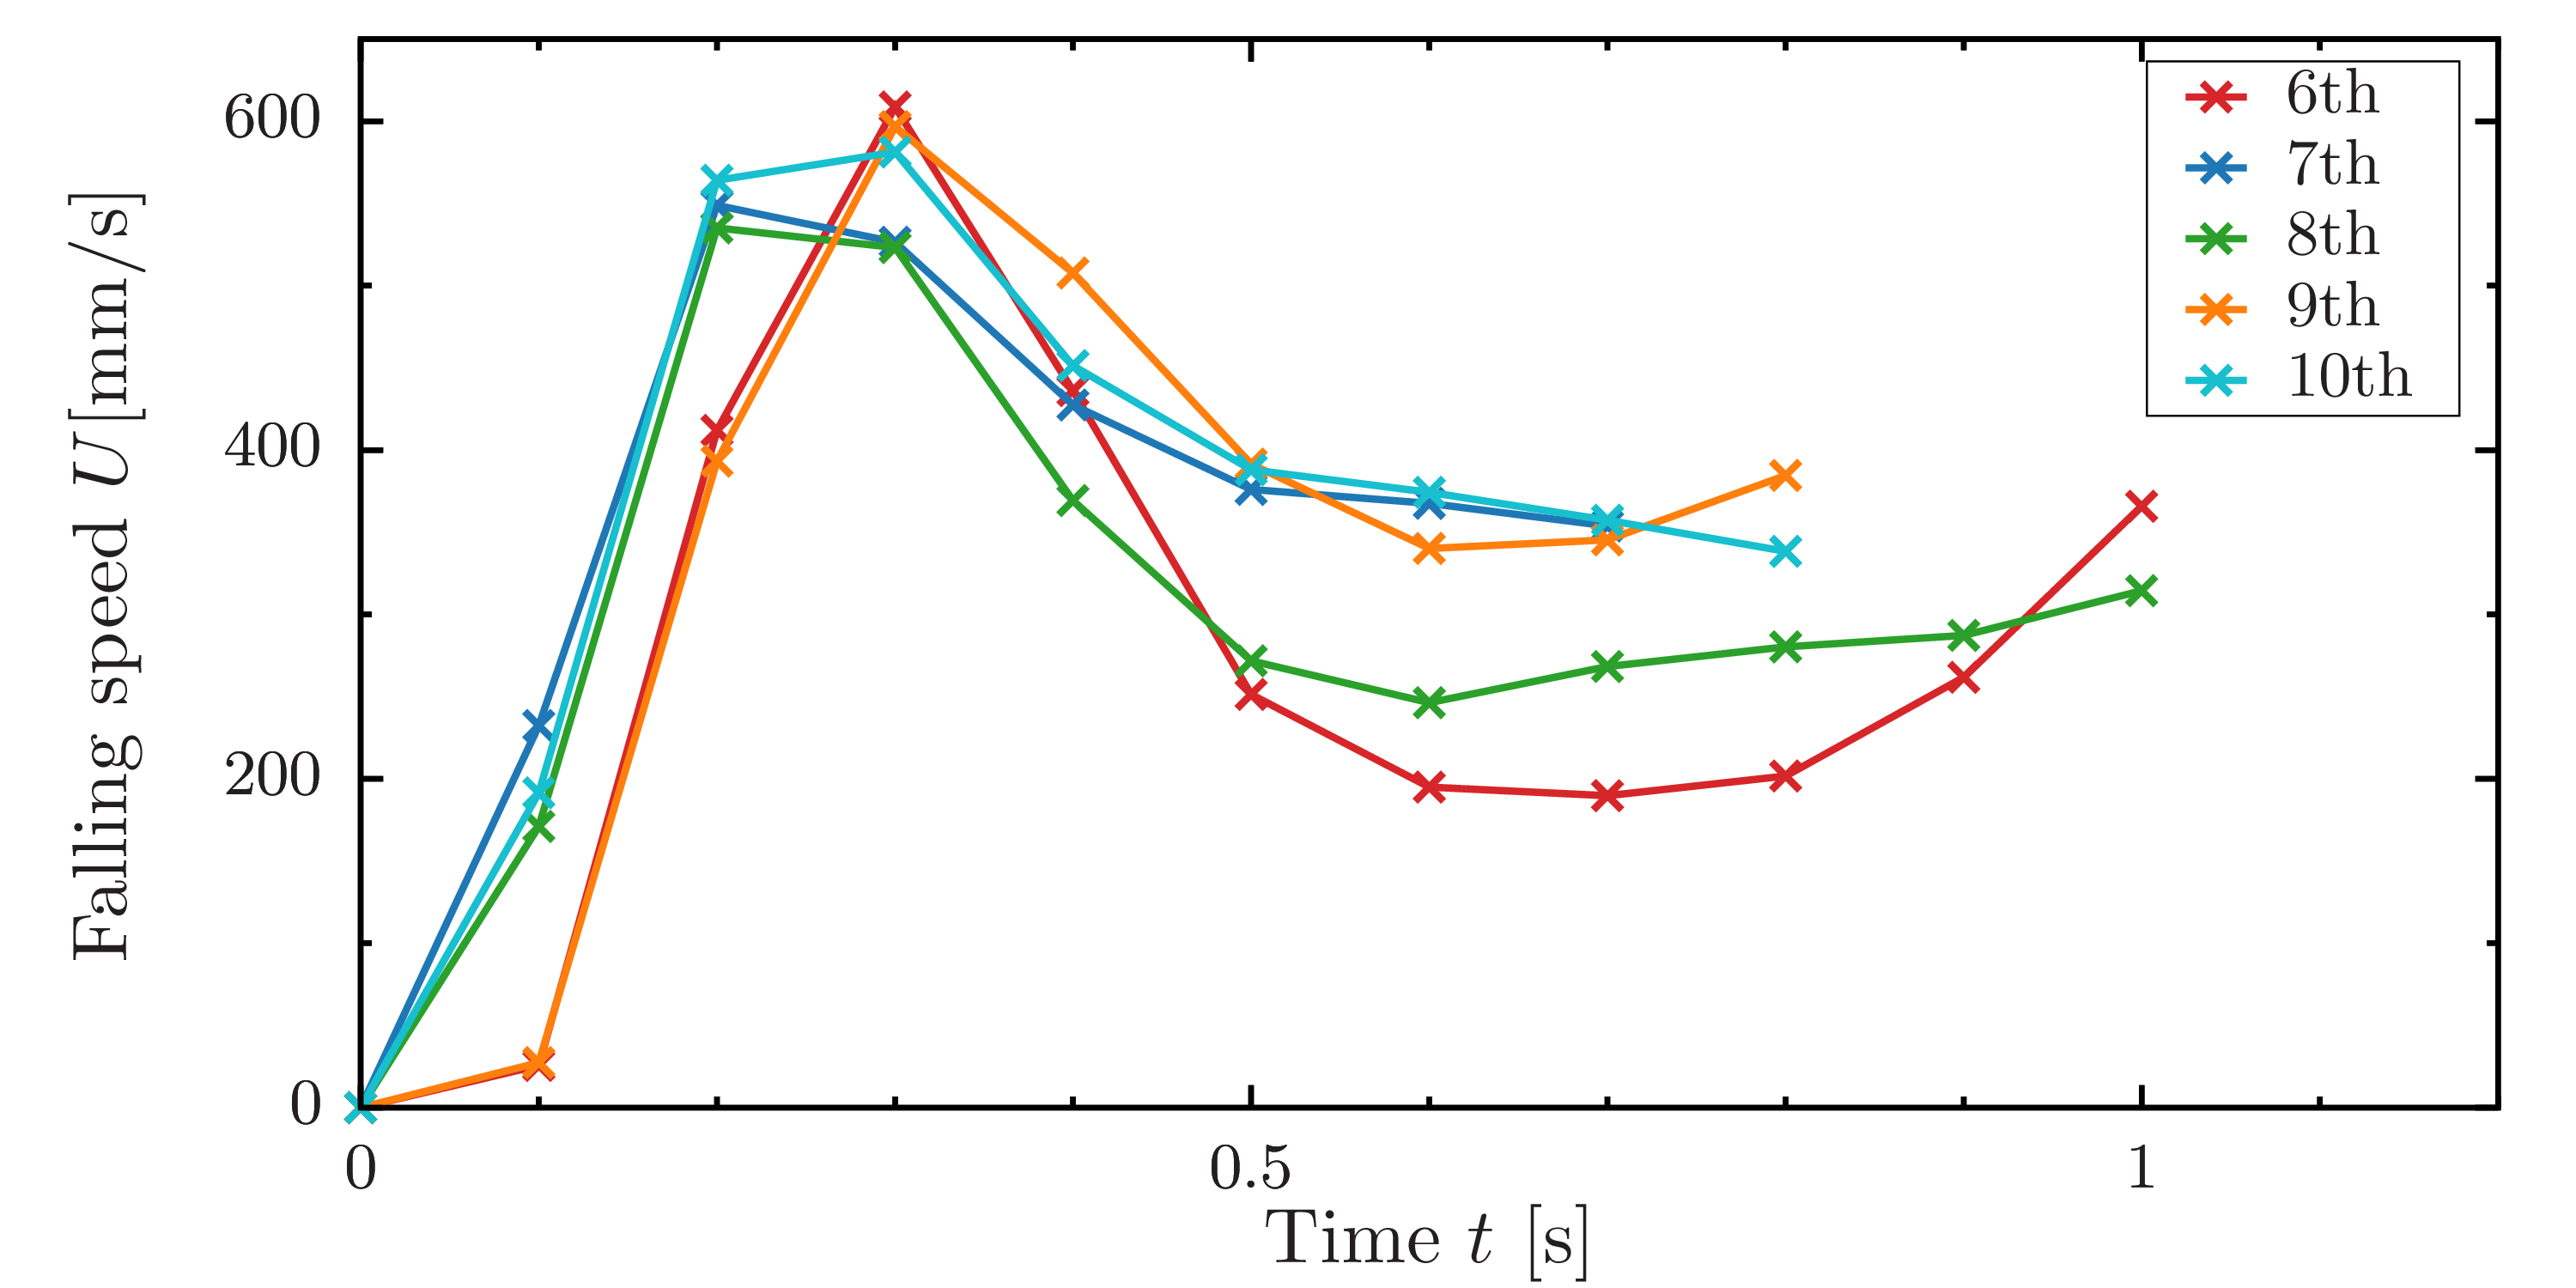
\includegraphics[width=12cm,clip]{4-Results/s0.5-39-6-10.png}
    \caption{Falling velocity of the sphere for each trial (\#6 to \#10) in 0.5wt.\%PAA solution with ultrasonic irradiation.}
    \label{fig:0.5onPAA-falling6-10}
\end{figure}

\clearpage

\subsubsection{1wt.\%PAA溶液}

1wt.\%PAA溶液中における球の落下速度を解析した結果をFig.\ref{fig:1PAA-falling}に示す.縦軸は落下速度,横軸は落下開始時からの経過時間である.先行研究であるIwamuro {\it et al.}\cite{ref:9}と比較して,超音波照射有無に関せず速度が増加している.これは粘度が低いためであると考えられる.また,超音波照射時における加速がIwamuro {\it et al.}\cite{ref:9}と比較して大きくなっている.このことは先述の4.2にて示した通り,今回形成された圧力場がより強いためであると考えられる.一方で,先行研究であるIwamuro {\it et al.}\cite{ref:9}と比較して,試行ごとのばらつきが大きくなった.

0.5wt.\%PAA溶液の場合と同様に,超音波照射なしの状態における1から5試行目の結果をFig.\ref{fig:1PAA-falling1-5}に,6から10試行目の結果をFig.\ref{fig:1PAA-falling6-10}に示す.先ほどの結果と同様に概ね試行回数を経るごとに球の落下速度が大きくなっていることが分かる.同様に,超音波照射ありの状態における1から5試行目の結果をFig.\ref{fig:1onPAA-falling1-5}に,6から10試行目の結果をFig.\ref{fig:1onPAA-falling6-10}に示す.先述の超音波なしの状態と同様に試行回数を経るごとに球の落下速度が大きくなっていることが分かった.

\begin{figure}[ht]
    \centering
    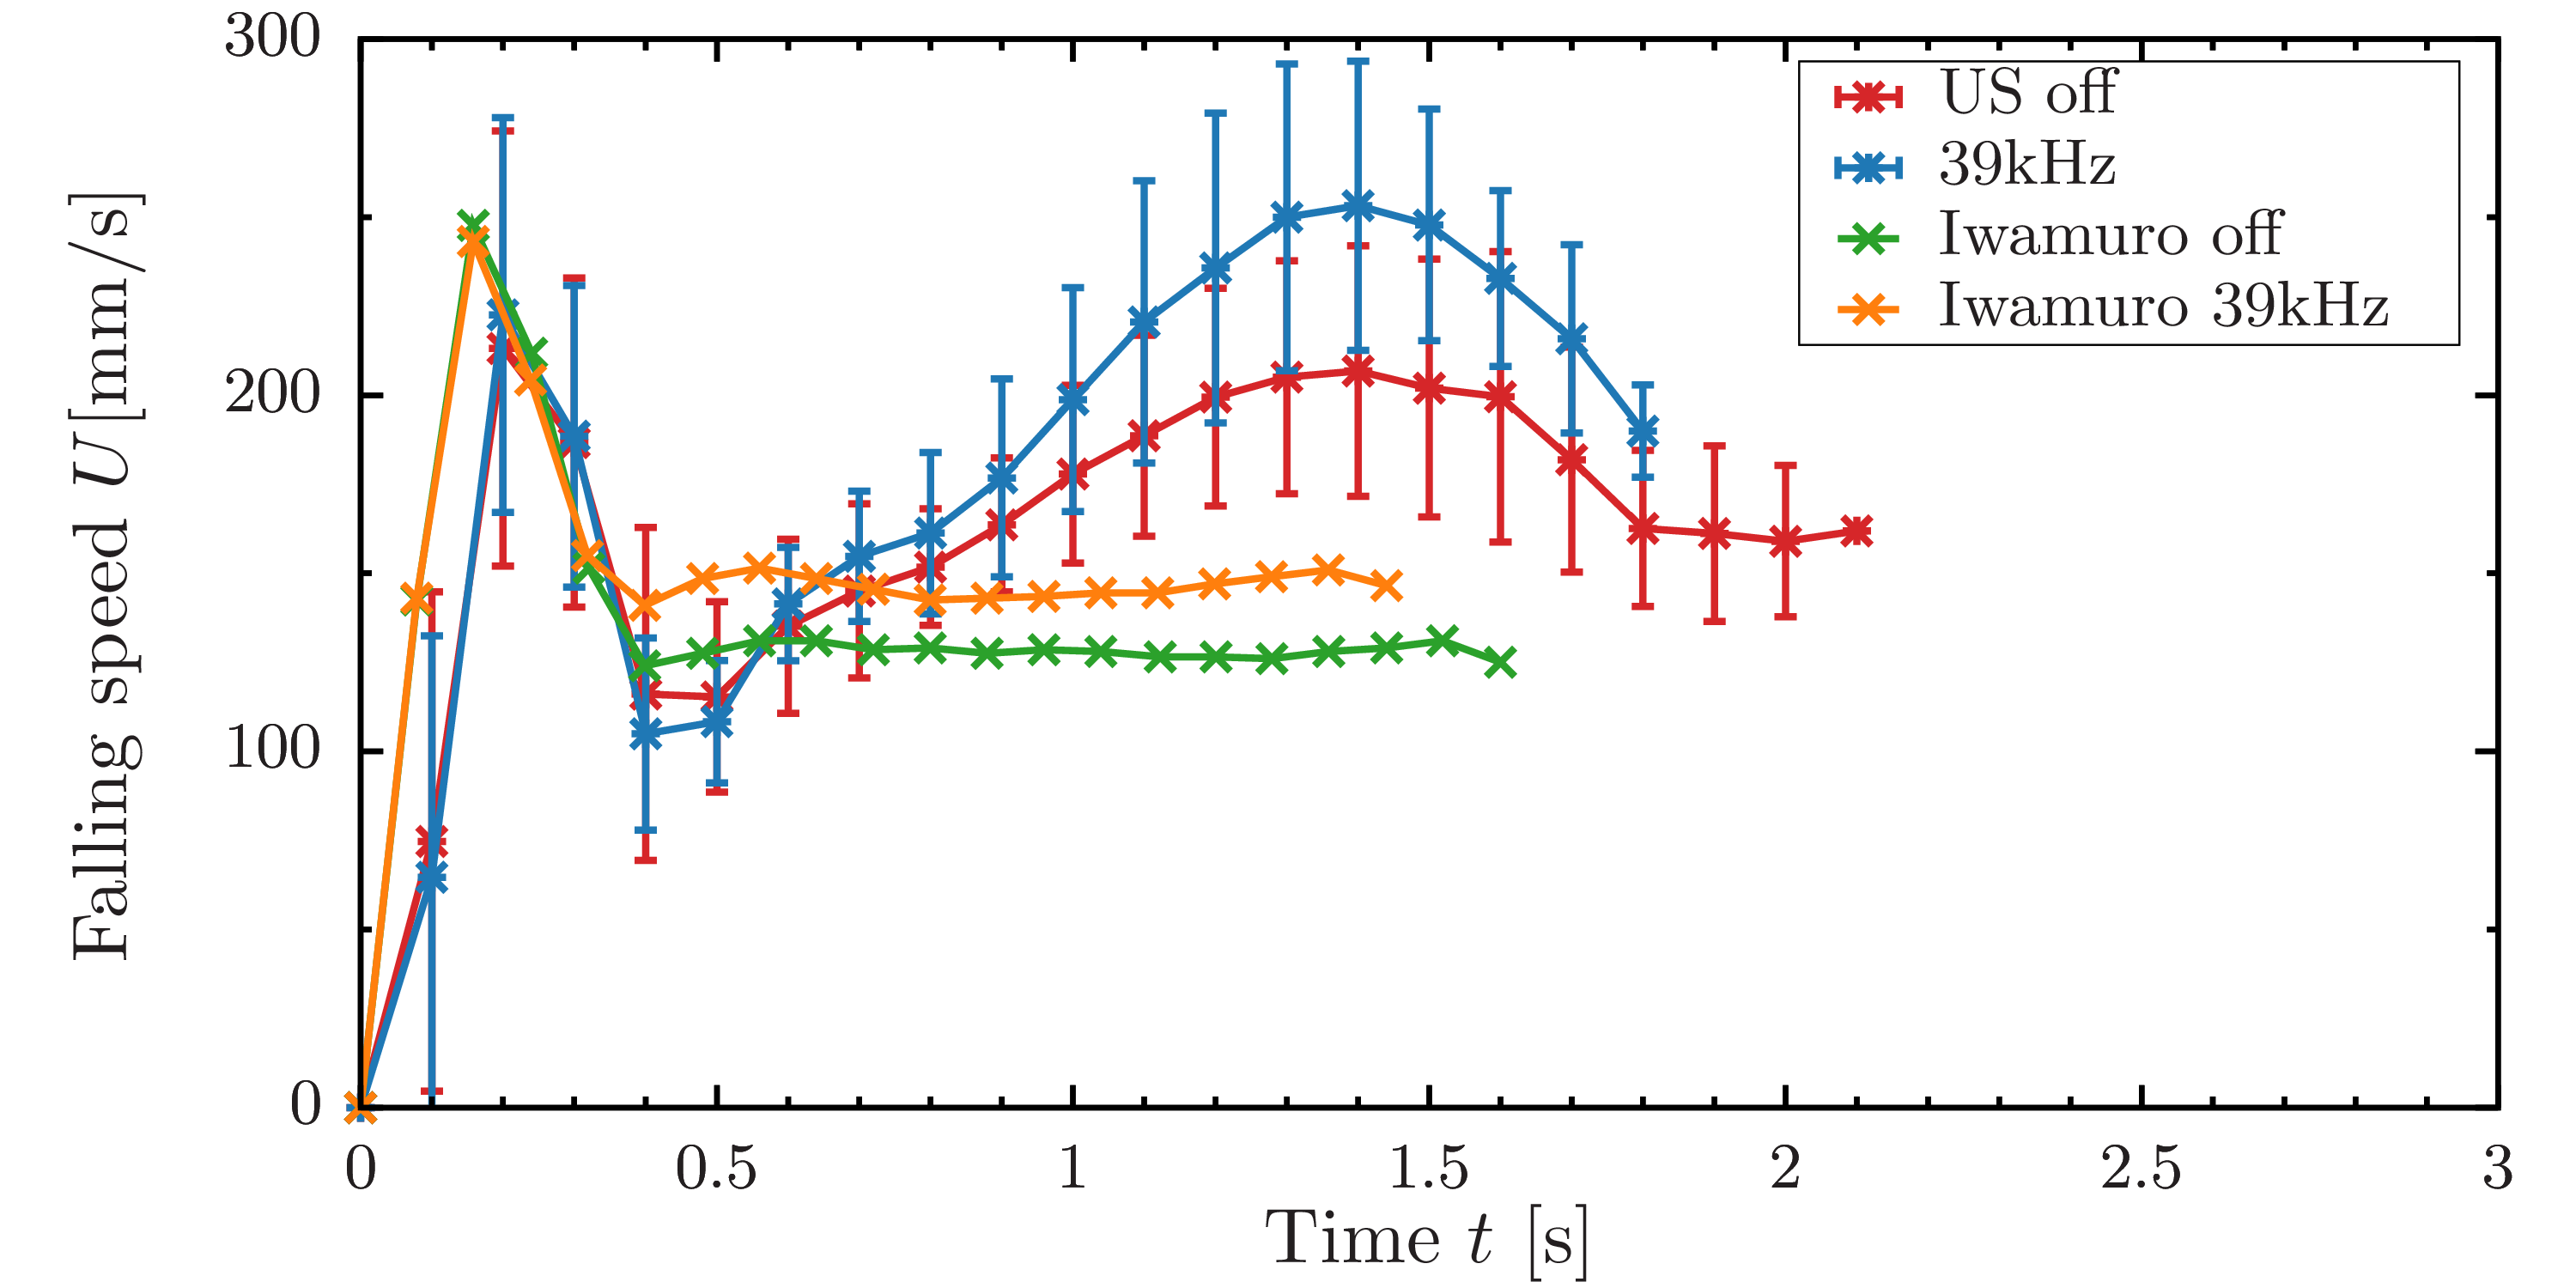
\includegraphics[width=12cm,clip]{./4-Results/s1.png}
    \caption{Falling velocity of a sphere in 1wt.\%PAA solution with and without ultrasound irradiation.}
    \label{fig:1PAA-falling}
    \centering
    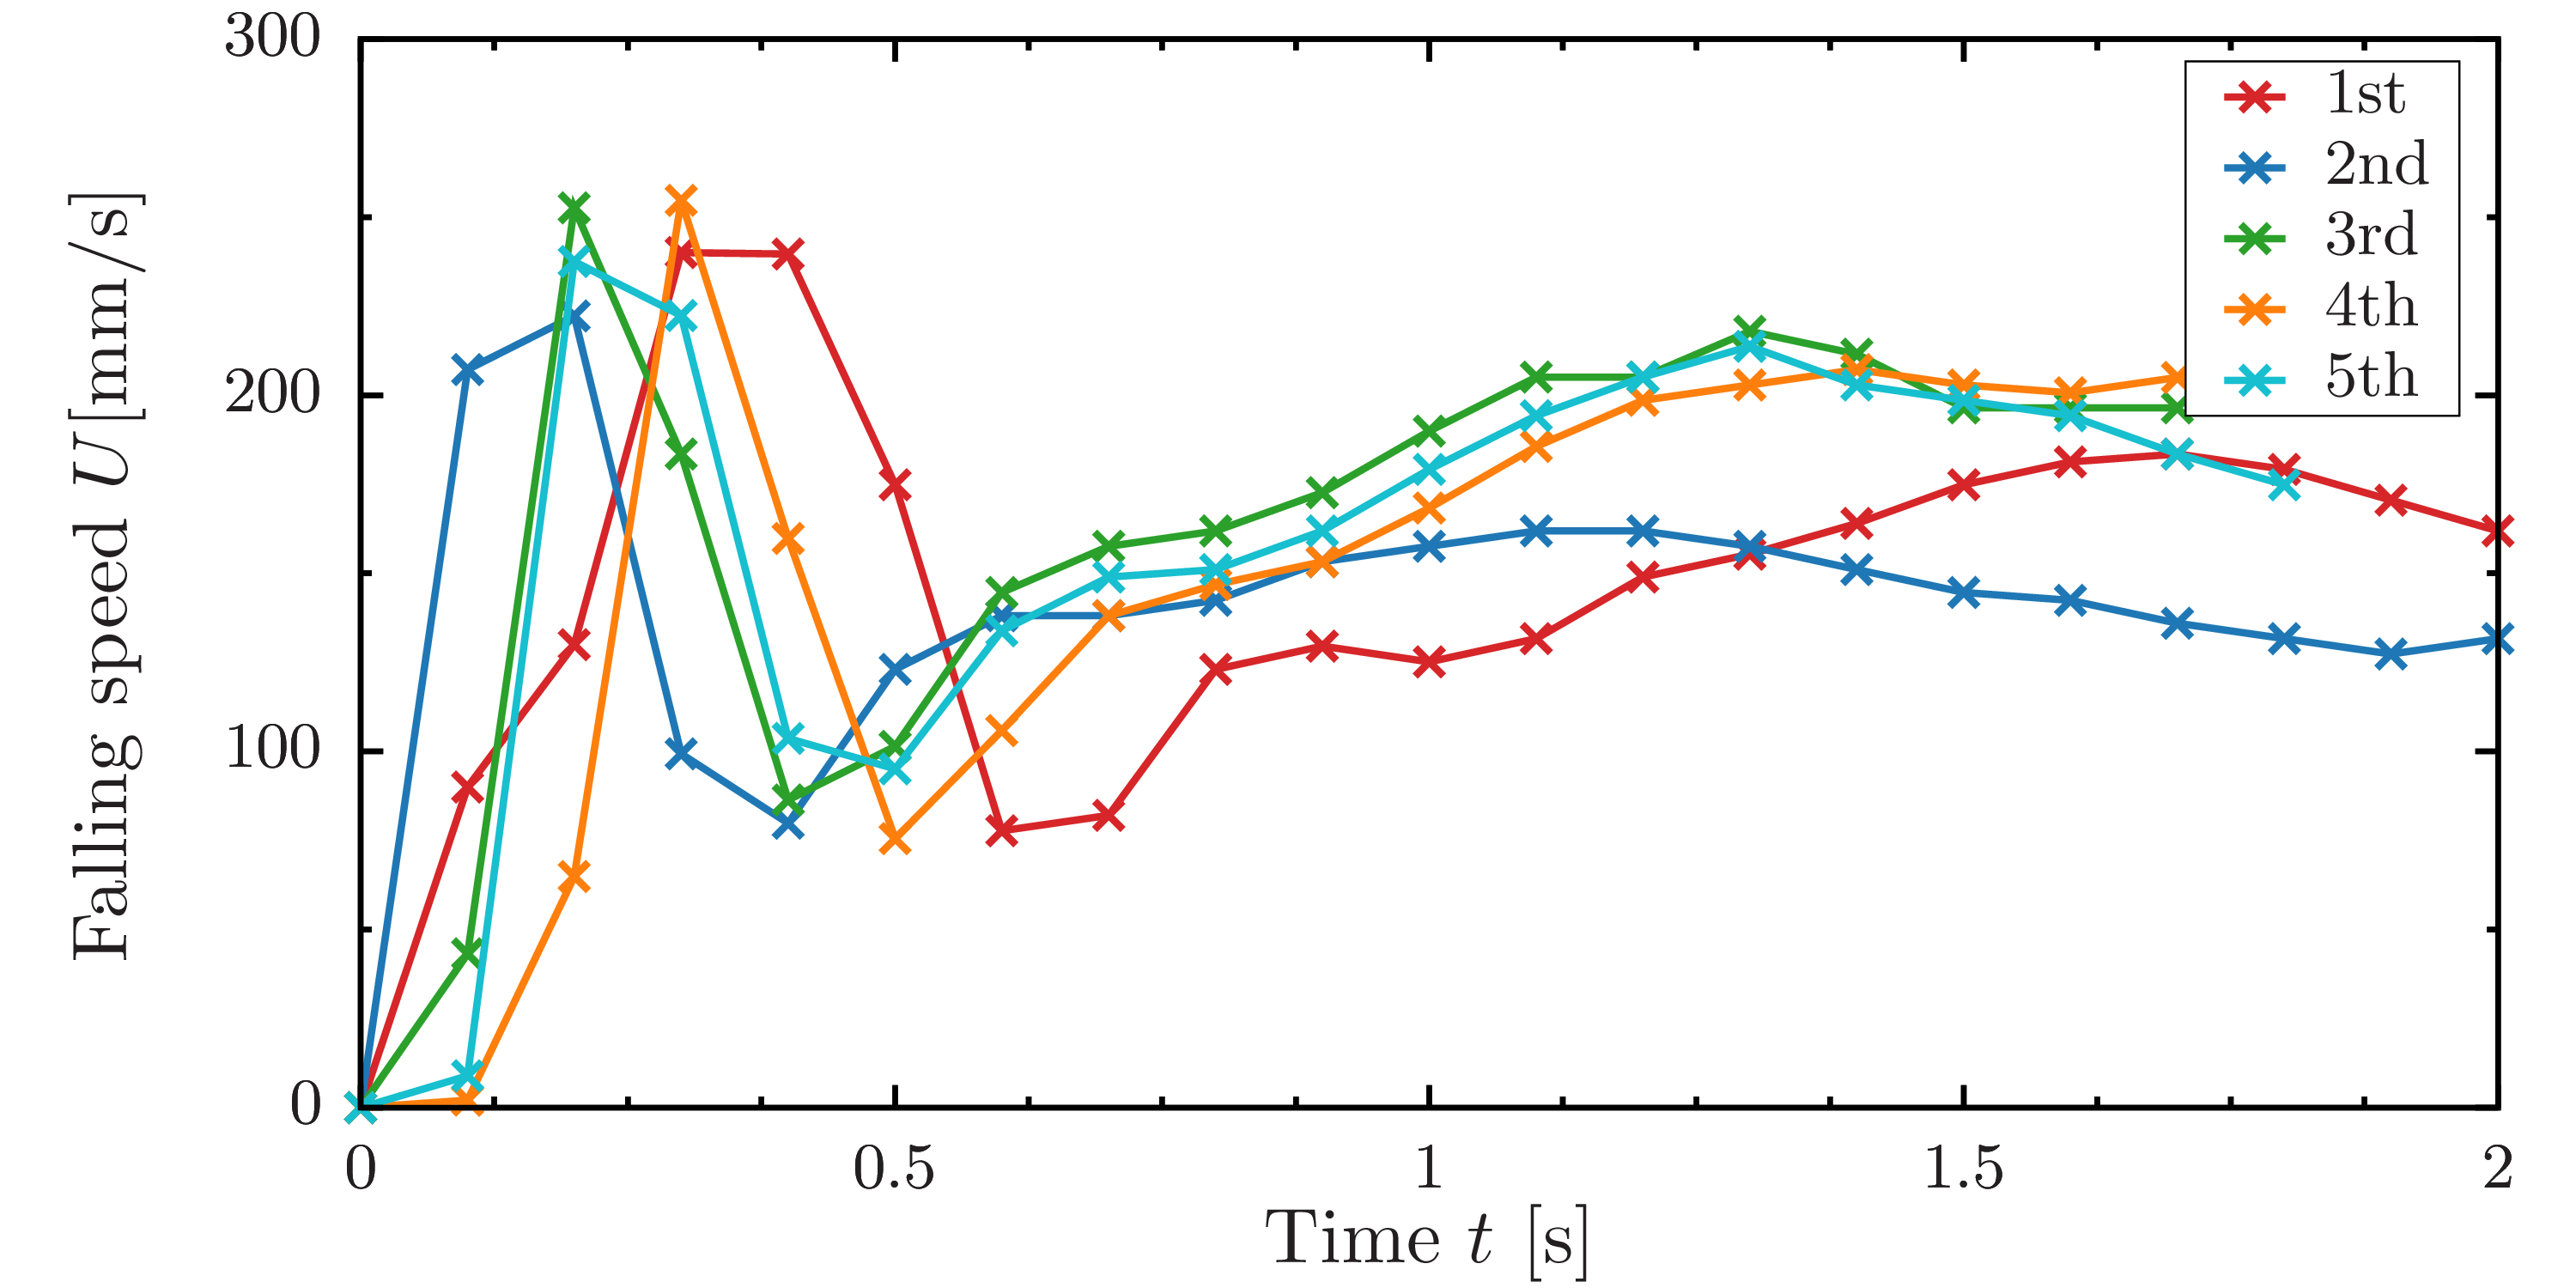
\includegraphics[width=12cm,clip]{4-Results/s1-1-5.png}
    \caption{Falling velocity of the sphere for each trial (\#1 to \#5) in 1wt.\%PAA solution without ultrasonic irradiation.}
    \label{fig:1PAA-falling1-5}
\end{figure}
\begin{figure}[ht]
    \centering
    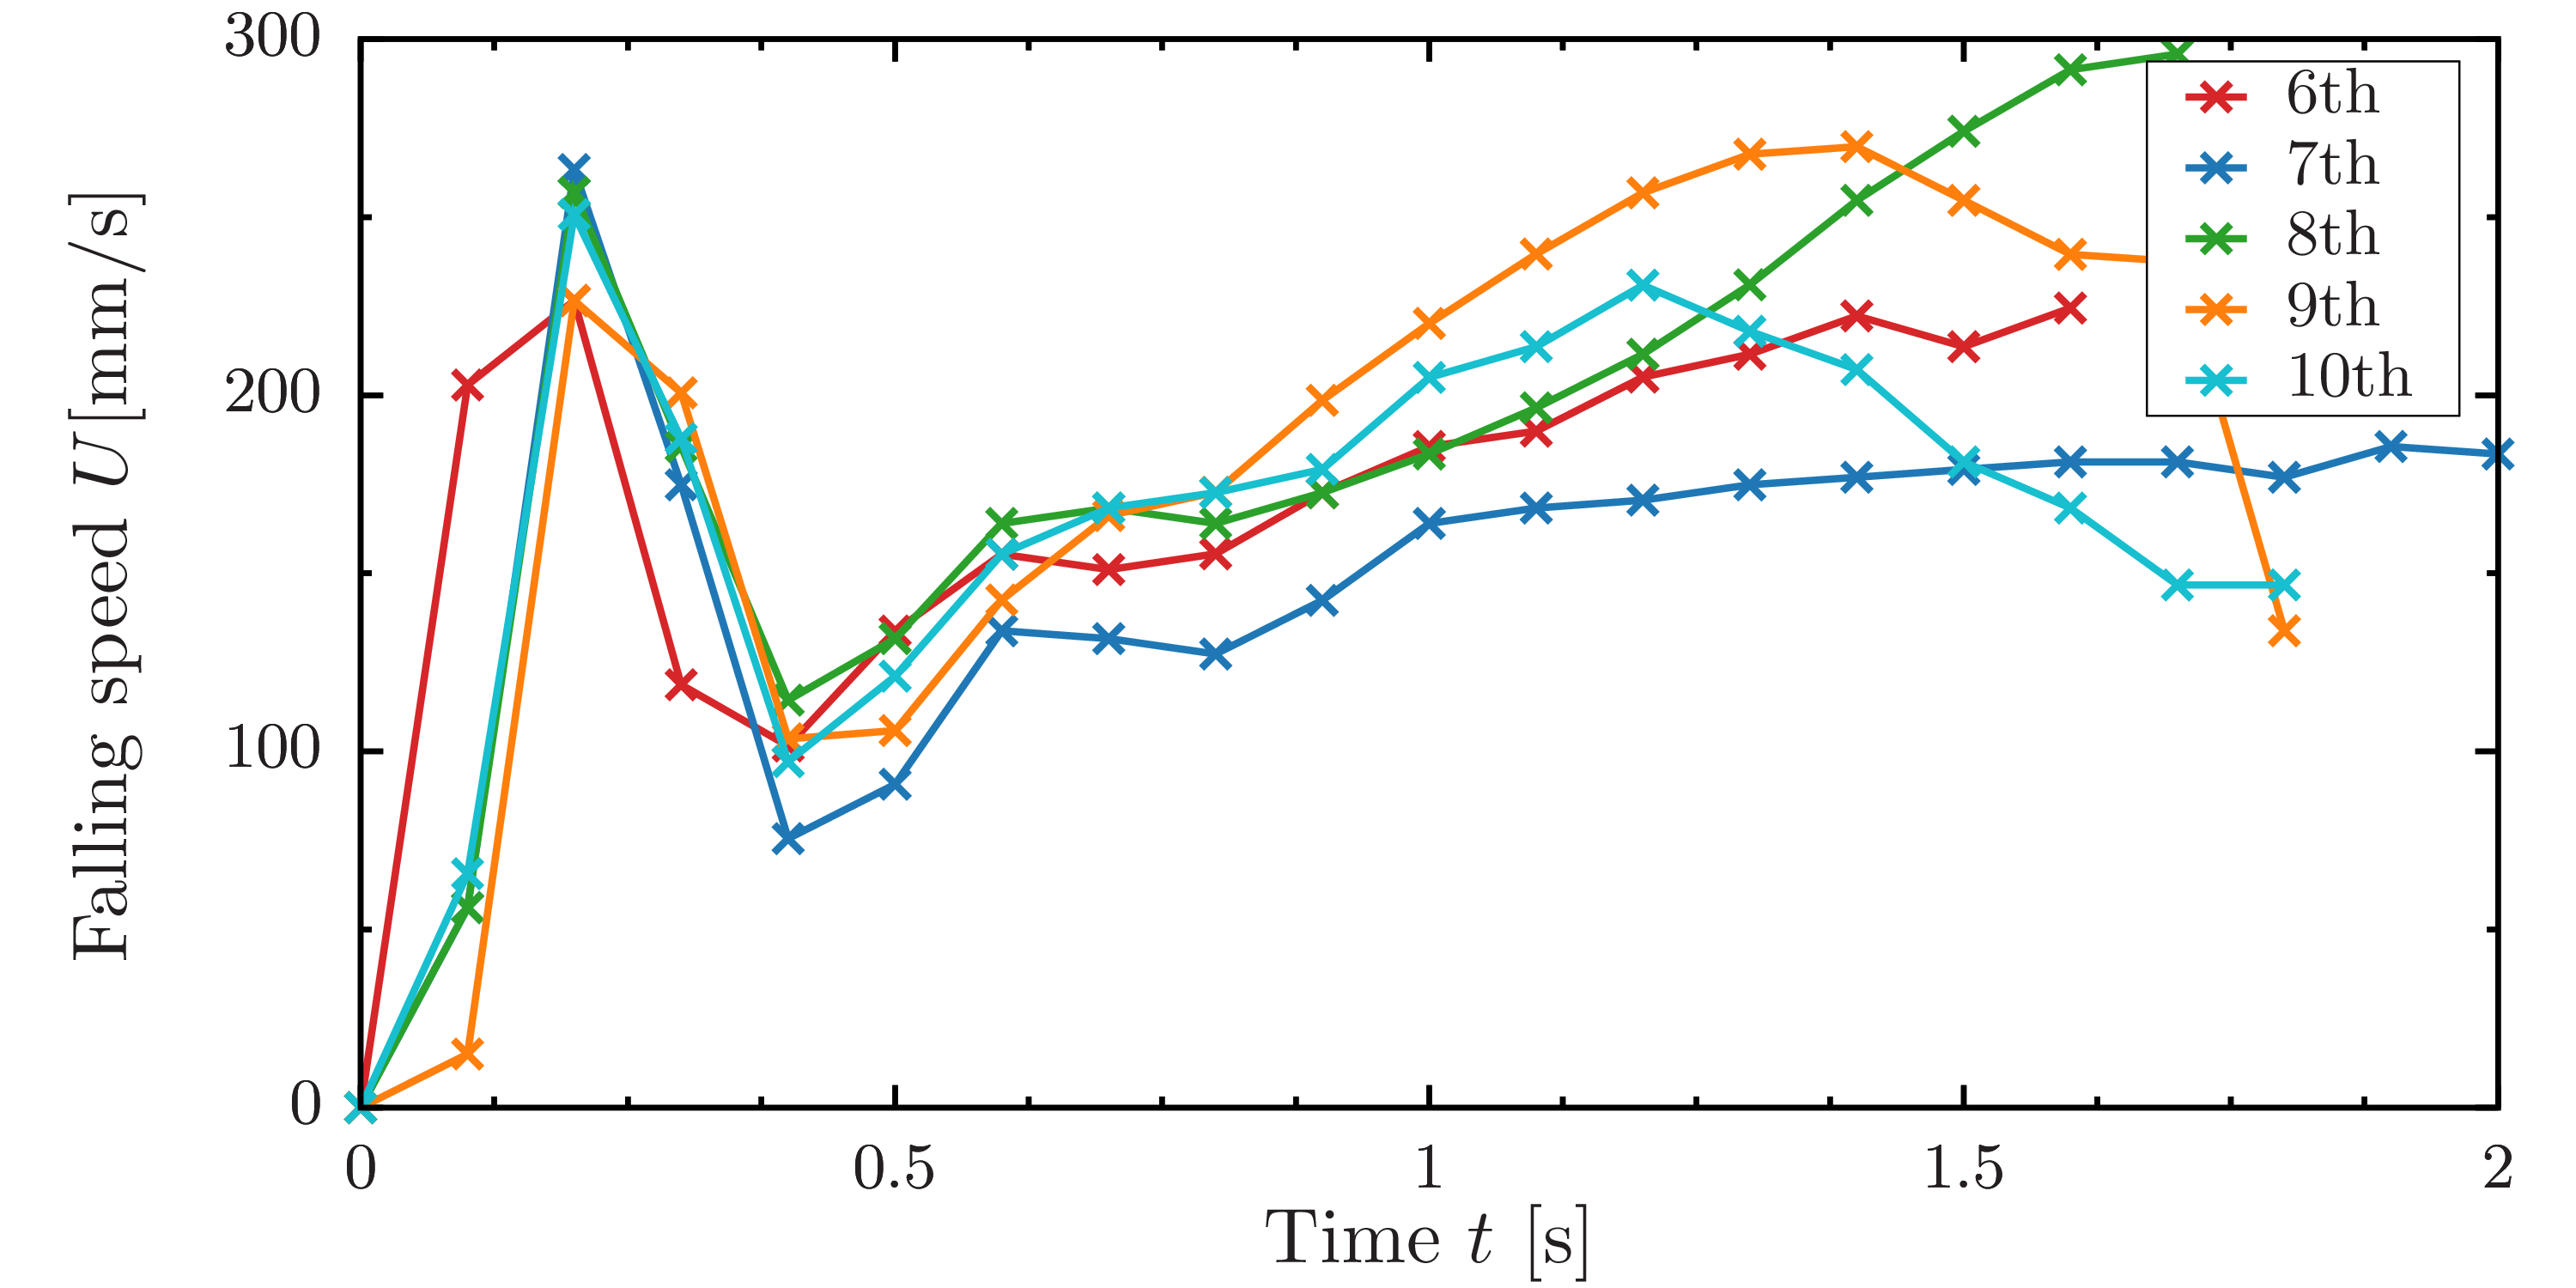
\includegraphics[width=12cm,clip]{4-Results/s1-6-10.png}
    \caption{Falling velocity of the sphere for each trial (\#6 to \#10) in 1wt.\%PAA solution without ultrasonic irradiation.}
    \label{fig:1PAA-falling6-10}
    \centering
    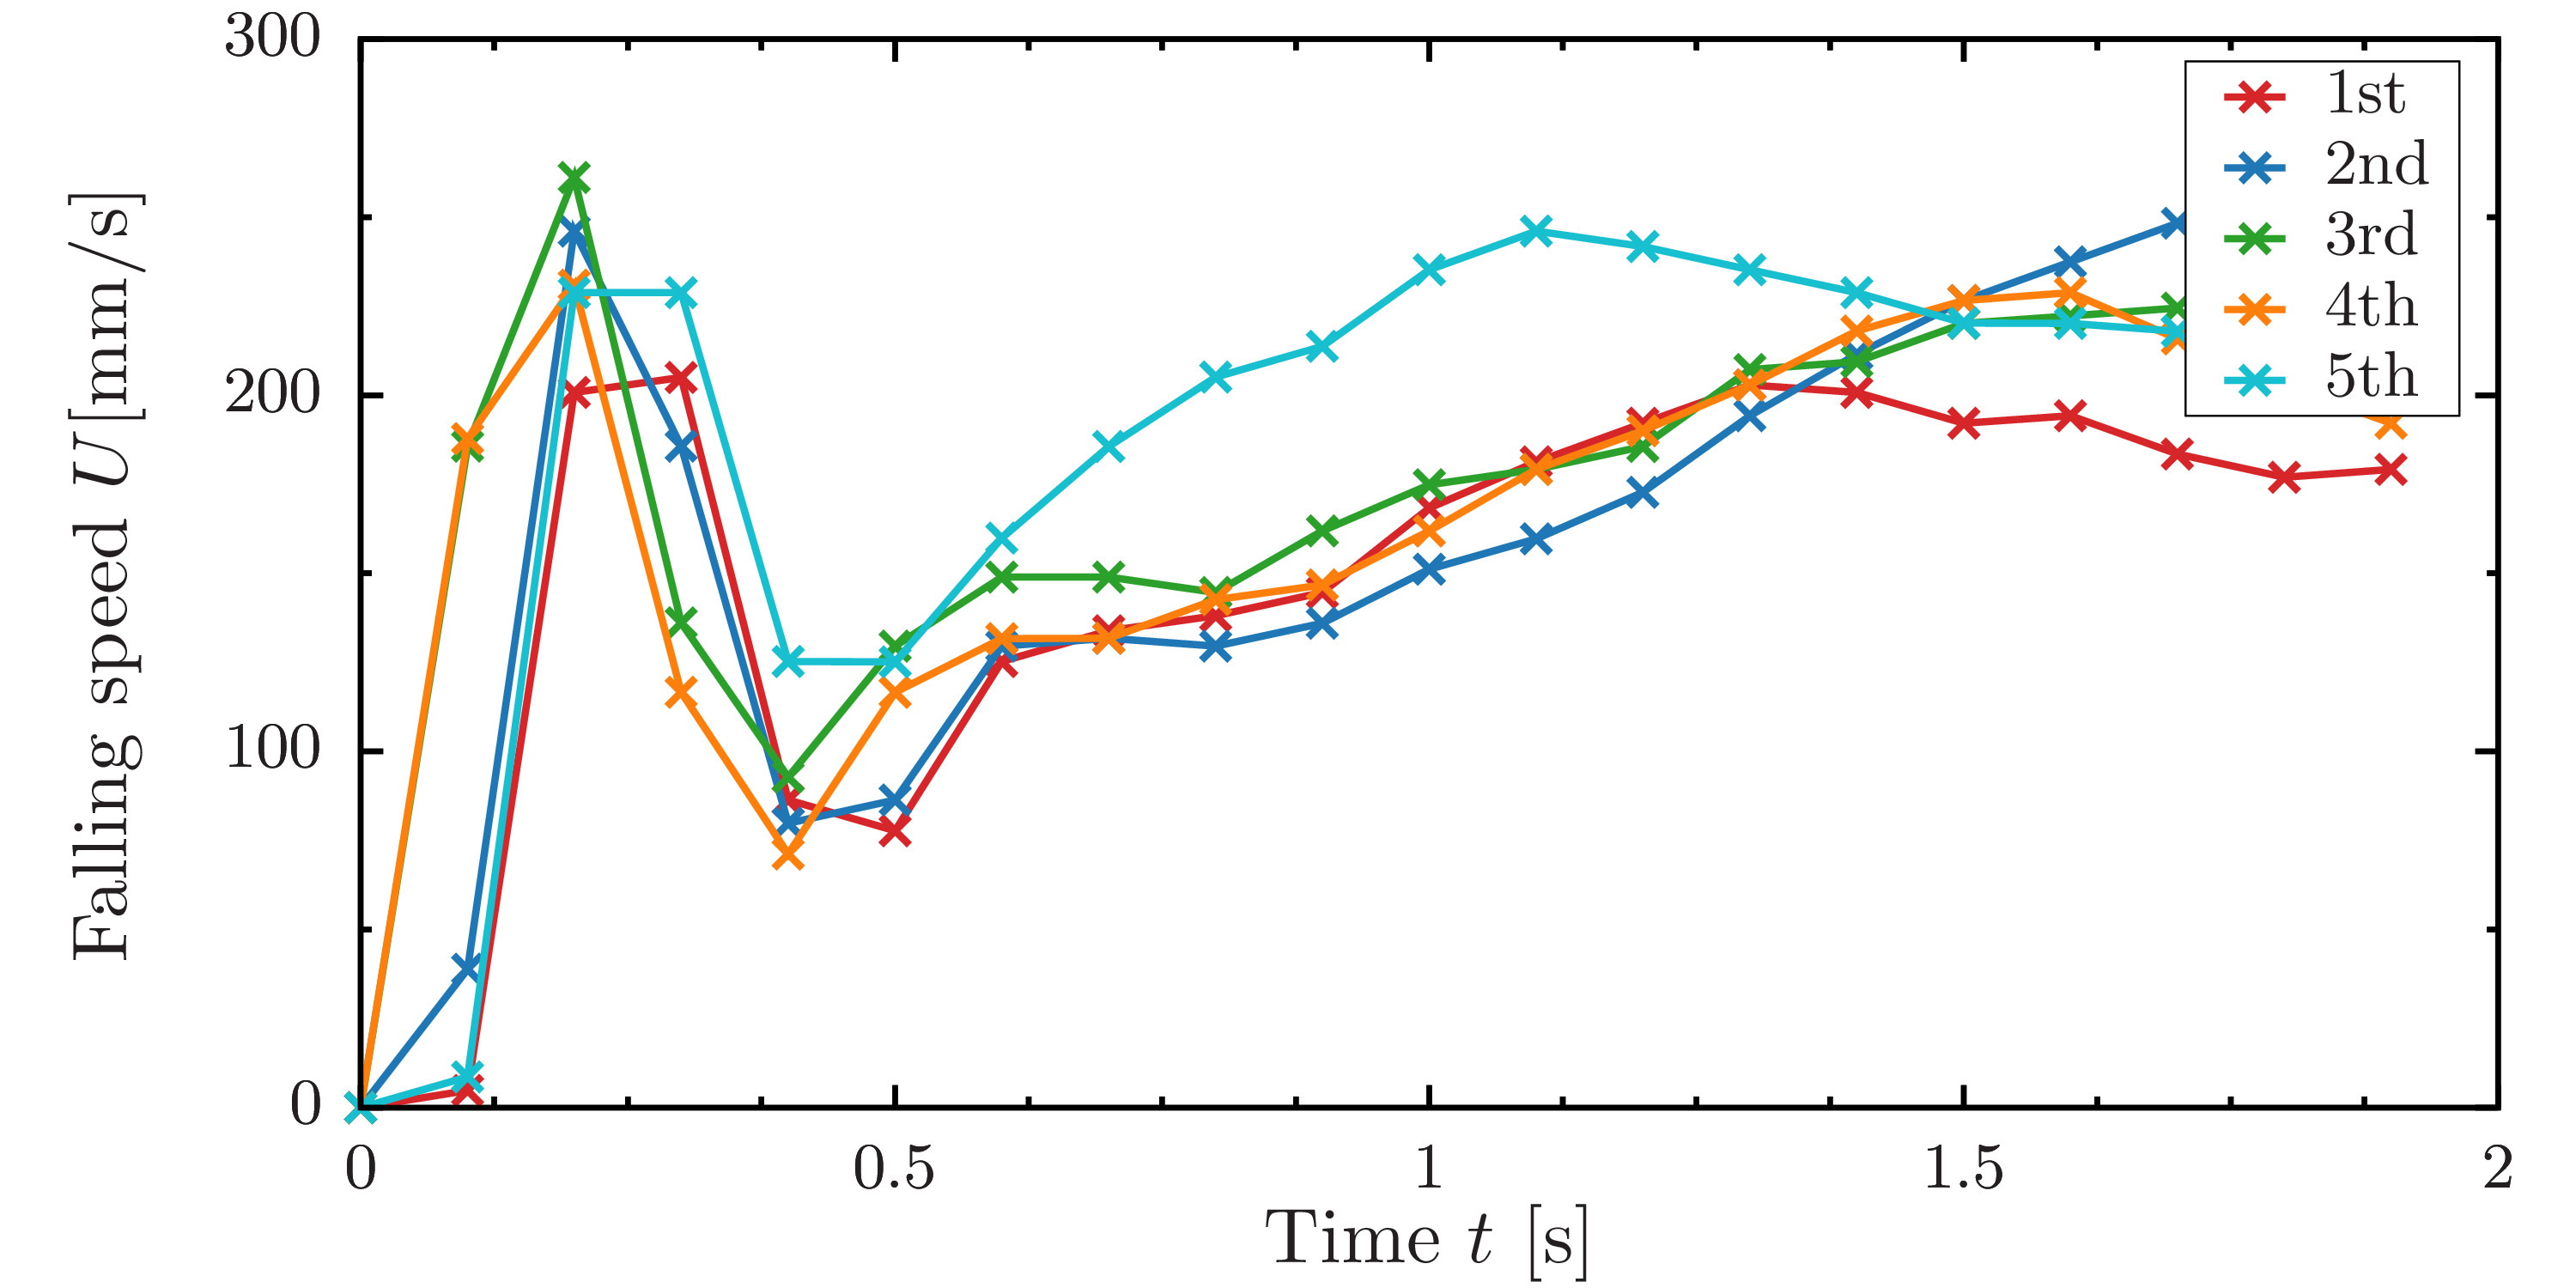
\includegraphics[width=12cm,clip]{4-Results/s1-39-1-5.png}
    \caption{Falling velocity of the sphere for each trial (\#1 to \#5) in 1wt.\%PAA solution with ultrasonic irradiation.}
    \label{fig:1onPAA-falling1-5}
    \centering
    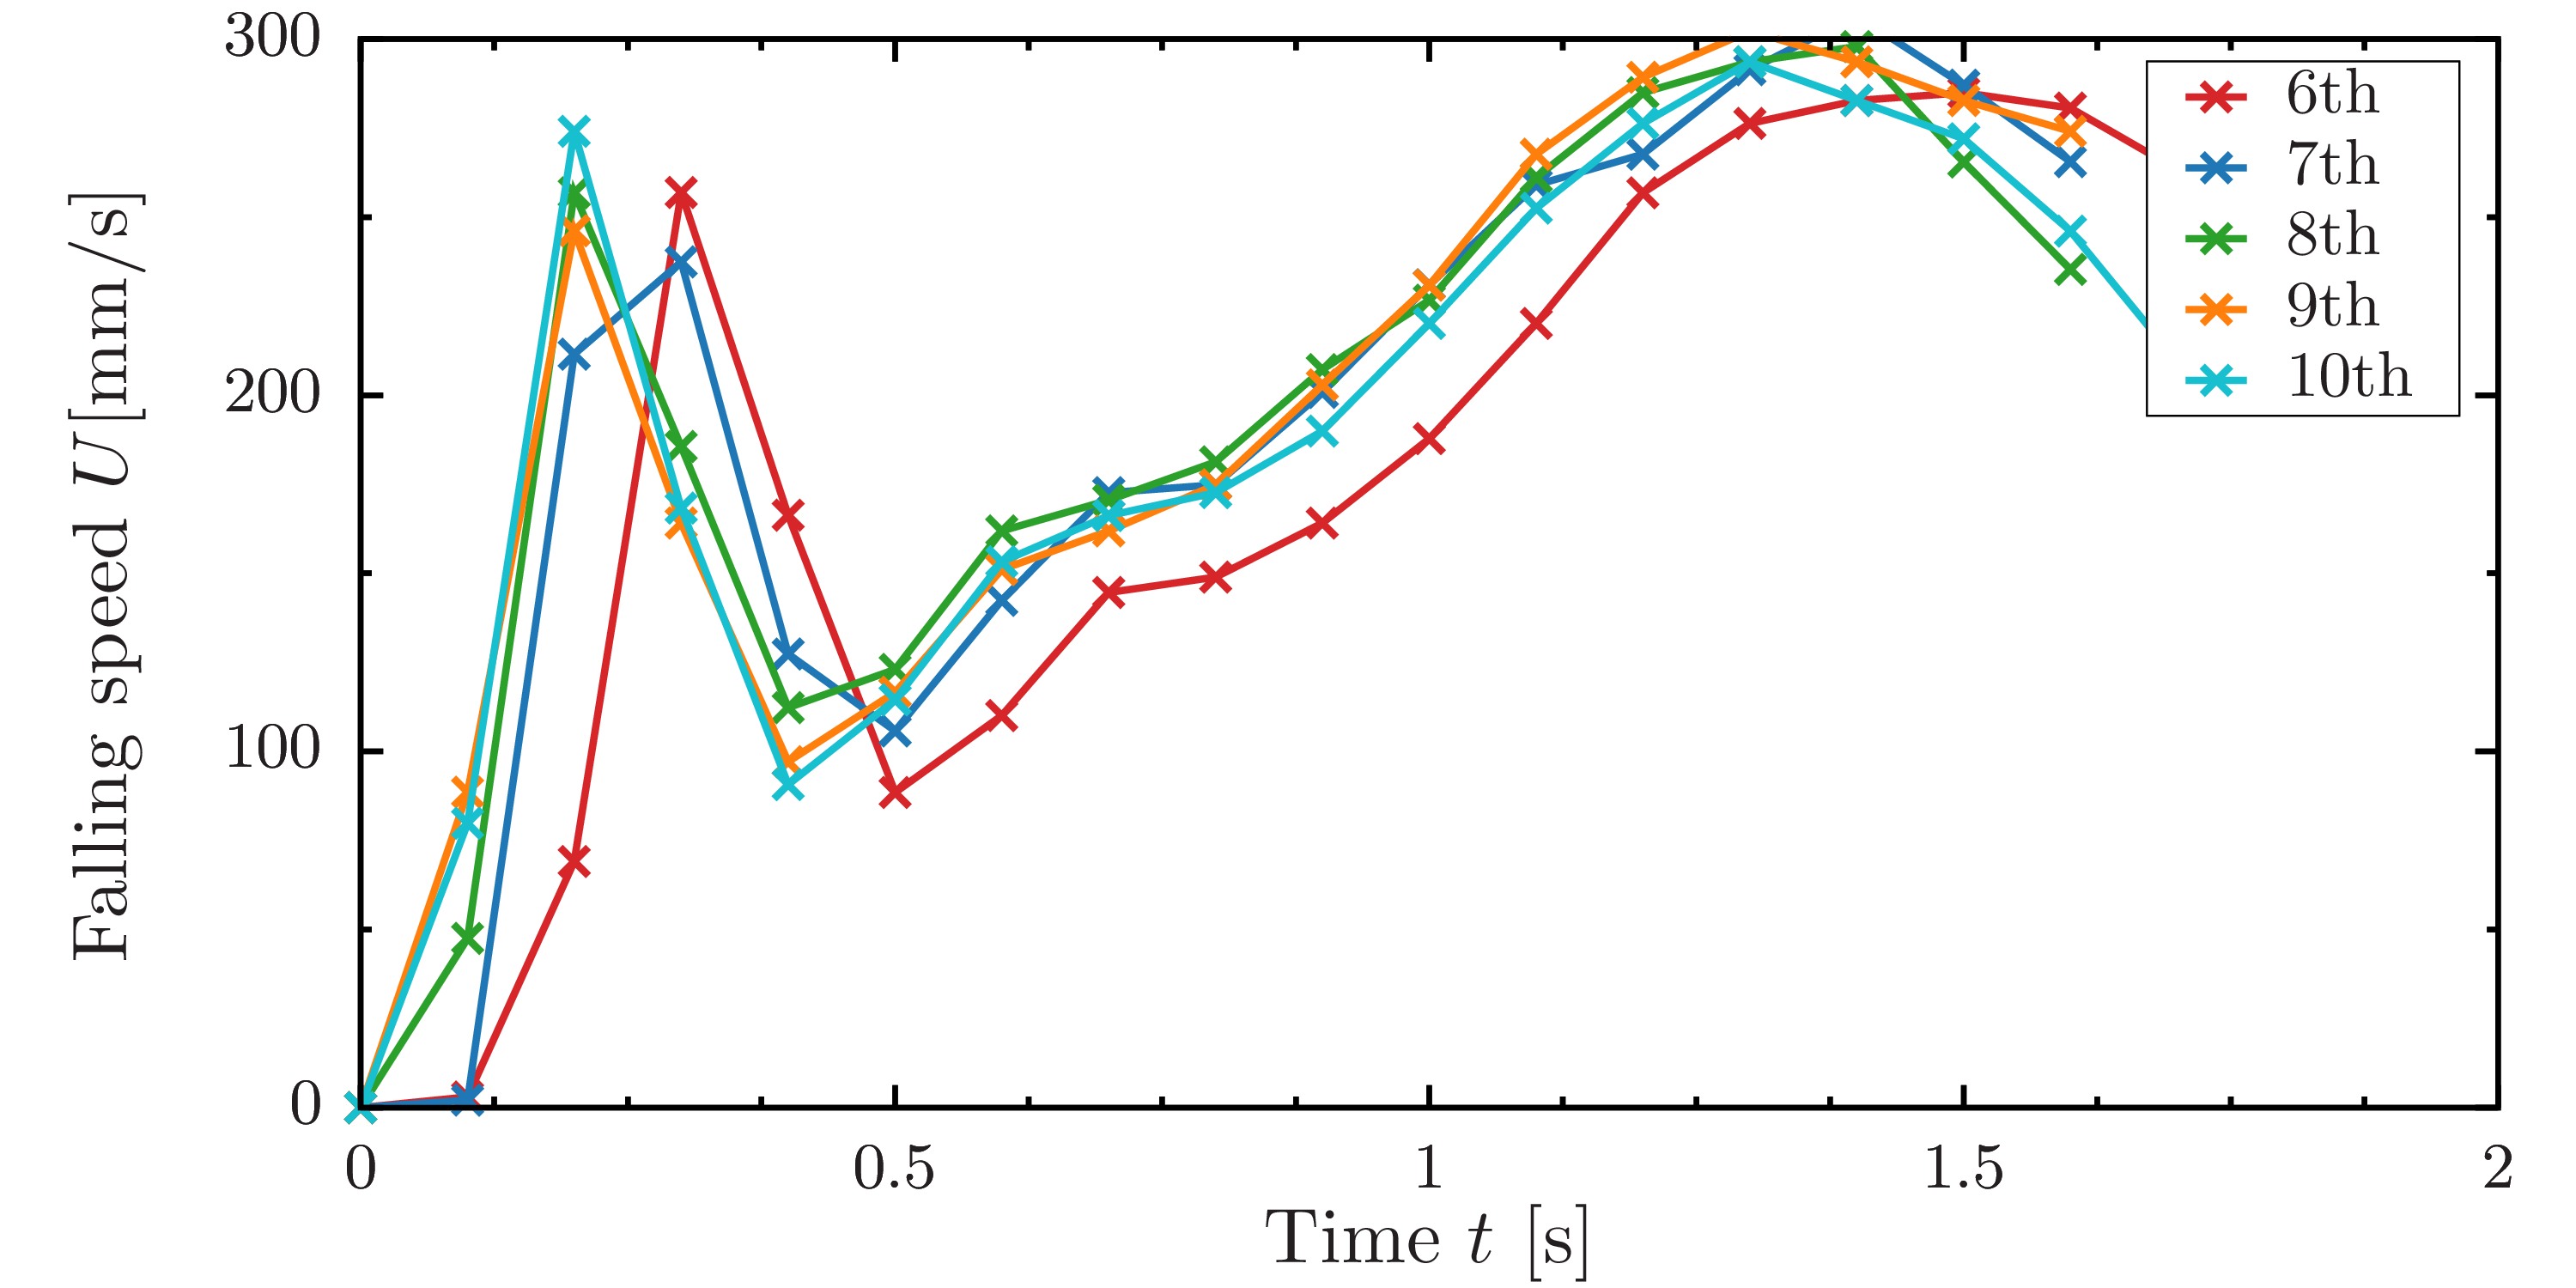
\includegraphics[width=12cm,clip]{4-Results/s1-39-6-10.png}
    \caption{Falling velocity of the sphere for each trial (\#6 to \#10) in 1wt.\%PAA solution with ultrasonic irradiation.}
    \label{fig:1onPAA-falling6-10}
\end{figure}
